\documentclass{article}

% --- PACKAGES (As provided from your Physics IA) ---
\usepackage[utf8]{inputenc}
\usepackage[T1]{fontenc}
\usepackage{amsmath}
\usepackage{amssymb} % Often useful for math symbols
\usepackage{graphicx}
\usepackage{siunitx}
\usepackage{booktabs}
\usepackage{hyperref}
\usepackage[margin=1in]{geometry}
\usepackage{fancyhdr} 
\usepackage{float} 
\usepackage{textgreek} 
\usepackage{listings} 
\usepackage{xcolor} 
% \usepackage{minted}

% --- DOCUMENT INFORMATION ---
\author{Candidate Name} % For header/footer purposes

% --- SIunitx Setup ---
\sisetup{detect-all}

% --- Code Listing Style Setup ---
\definecolor{codegreen}{rgb}{0,0.6,0}
\definecolor{codegray}{rgb}{0.5,0.5,0.5}
\definecolor{codepurple}{rgb}{0.58,0,0.82}
\definecolor{backcolour}{rgb}{0.95,0.95,0.92}

\lstdefinestyle{mystyle}{
    backgroundcolor=\color{backcolour},   
    commentstyle=\color{codegreen},
    keywordstyle=\color{magenta},
    numberstyle=\tiny\color{codegray},
    stringstyle=\color{codepurple},
    basicstyle=\ttfamily\footnotesize,
    breakatwhitespace=false,         
    breaklines=true,                 
    captionpos=b,                    
    keepspaces=true,                 
    numbers=left,                    
    numbersep=5pt,                  
    showspaces=false,                
    showstringspaces=false,
    showtabs=false,                  
    tabsize=2
}
\lstset{style=mystyle}


% --- FOOTER AND HEADER SETUP ---
\pagestyle{fancy}
\fancyhf{} % Clear all header and footer fields

\fancyfoot[C]{\thepage} 
\fancyfoot[R]{Fourier Analysis of Timbre} % Short title
\renewcommand{\headrulewidth}{0pt}
\renewcommand{\footrulewidth}{0.4pt}

% ======================================================================
% --- BEGIN DOCUMENT ---
% ======================================================================

\begin{document}

% --- TITLE PAGE ---
\begin{titlepage}
    \centering
    \vspace*{2cm}
    
    \Large{\textbf{Mathematics: Analysis and Approaches}}
    \vspace{0.5cm}
    
    \Large{\textbf{Internal Assessment}}
    \vspace{3cm}
    
    \huge{\textbf{Applying the Discrete Fourier Transform to Decompose, Analyze, and Reconstruct the Harmonic Structure of a Plucked Guitar String}}
    \vspace{5cm}
    
    \Large{Page Count: 18       }
    
    \vfill
    
    \Large{\today}
\end{titlepage}

\newpage

% --- INTRODUCTION ---
\section{Introduction}

\subsection{Context and Rationale}
When I play or listen to a guitar, I don’t just hear “a note.” I hear a sound with a texture, something fuller than a single pitch. That texture is what musicians call timbre, and it’s usually described in vague words like warm or bright. I wanted to see if there’s a way to strip away the vague part and capture that sound in actual numbers.

I decided to take a single recorded guitar note and study it. Instead of thinking of the note as one pitch, it can be broken down into a fundamental frequency and a set of harmonics layered on top of it. Those layers are what give the guitar its voice. My initial curiosity about this decomposition was solidified by the visual intuition provided by sources like 3Blue1Brown's work on Fourier series, which helped bridge the gap between the abstract formula and the tangible quality of a sound I could hear \cite{3b1b}.

Fourier analysis is the tool that can do this breakdown. By applying it, I can check whether the messy waveform of the guitar can be reconstructed from simpler sinusoidal pieces. If it works, the result is not just a match between graphs, it’s a measurable “fingerprint” of that warm feeling you hear, i.e timbre. That’s what makes this worth exploring, and it leads directly into the research question that follows.

\subsection{Research Question}
To what extent can a recorded guitar note be accurately reconstructed using a complex Fourier series, and how does its harmonic structure explain the timbre of the instrument?

\subsection{Theoretical Framework}
Before testing the idea, I needed to build the mathematical model from the ground up. This involved starting with the physics of a sound wave, deriving the tools to analyze it, and then refining those tools into a final, testable hypothesis.

    \subsubsection{Justifying the Model: The Wave Equation and Superposition}

To begin rigorously, I model a vibrating guitar string of length $L$. Its transverse displacement $u(x,t)$ 
satisfies the one-dimensional wave equation\footnote{The physical derivation of the wave equation for a vibrating string is a fundamental application of Newton's second law to continuous media, a topic standard in university-level physics and mechanics literature \cite{halliday_resnick}.}
\begin{equation}
    \frac{\partial^2 u}{\partial t^2}(x,t) = c^2 \frac{\partial^2 u}{\partial x^2}(x,t), 
    \label{eq:wave}
\end{equation}
where $c$ is the wave speed, determined by the string’s tension and density. This is a \emph{partial differential equation} (PDE) because it involves derivatives in both space $x$ and time $t$. The following derivation is a standard approach found in mathematical physics literature \cite{stein2003fourier}.

To ensure clarity throughout the derivation, the key variables and constants are defined as follows:
\begin{itemize}
    \item $u(x,t)$ is the transverse displacement of the string at position $x$ and time $t$.
    \item $c$ is the wave speed along the string.
    \item $L$ is the total length of the vibrating string.
    \item $n$ is a positive integer representing the harmonic number ($n=1$ is the fundamental, $n=2$ is the first overtone, etc.).
    \item $\lambda_n$ is the spatial eigenvalue for the $n$-th harmonic.
    \item $\omega_n$ is the angular frequency of the $n$-th harmonic.
\end{itemize}

\paragraph{Separation of Variables.} 
To solve \eqref{eq:wave}, I assume a separable solution of the form
\begin{equation}
    u(x,t) = X(x)T(t),
\end{equation}
where $X$ depends only on $x$ and $T$ depends only on $t$. To substitute this back into the wave equation, I first calculate the second-order partial derivatives with respect to time $t$ and space $x$:
\begin{align}
    \frac{\partial^2 u}{\partial t^2} &= X(x)T''(t), \\
    \frac{\partial^2 u}{\partial x^2} &= X''(x)T(t).
\end{align}
Substituting these calculated derivatives into \eqref{eq:wave} yields
\begin{equation}
    X(x) T''(t) = c^2 X''(x) T(t).
\end{equation}
Dividing through by $c^2 X(x)T(t)$ (assuming $X,T \neq 0$) isolates the time-dependent and space-dependent terms:
\begin{equation}
    \frac{T''(t)}{c^2 T(t)} = \frac{X''(x)}{X(x)}.
\end{equation}

The left-hand side is a function of $t$ only, while the right-hand side is a function of $x$ only. For equality to hold for \emph{all} $x$ and $t$, both sides must equal a constant. I denote this constant by $-\lambda^2$, since a negative value ensures oscillatory (sinusoidal) solutions rather than exponential growth or decay:
\begin{equation}
    \frac{T''(t)}{c^2 T(t)} = \frac{X''(x)}{X(x)} = -\lambda^2.
\end{equation}

This reduces the PDE into two ordinary differential equations (ODEs):
\begin{align}
    X''(x) + \lambda^2 X(x) &= 0, \label{eq:Xode}\\
    T''(t) + c^2 \lambda^2 T(t) &= 0. \label{eq:Tode}
\end{align}

\paragraph{Solving the spatial equation.}
Equation \eqref{eq:Xode} has characteristic equation $r^2 + \lambda^2 = 0$, whose solutions are $r = \pm i\lambda$. Thus the general solution is
\begin{equation}
    X(x) = C \cos(\lambda x) + D \sin(\lambda x).
\end{equation}
For a string fixed at both ends, $u(0,t)=u(L,t)=0$, which implies $X(0)=0$ and $X(L)=0$. Applying $X(0)=0$ forces $C=0$. Then
\begin{equation}
    X(x) = D \sin(\lambda x).
\end{equation}
Applying $X(L)=0$ requires $\sin(\lambda L)=0$, hence
\begin{equation}
    \lambda L = n\pi, \qquad n=1,2,3,\dots
\end{equation}
and therefore the allowed spatial modes are
\begin{equation}
    X_n(x) = \sin\!\left(\frac{n\pi x}{L}\right).
\end{equation}

\paragraph{Solving the temporal equation.}
For each $\lambda_n = \tfrac{n\pi}{L}$, the time equation \eqref{eq:Tode} becomes
\begin{equation}
    T''(t) + \omega_n^2 T(t) = 0, \qquad \omega_n = \frac{n\pi c}{L}.
\end{equation}
To solve this second-order linear ordinary differential equation, I set up the characteristic equation\footnote{Solving homogeneous linear differential equations using characteristic equations relies on polynomial root-finding techniques, aligning with the complex polynomial algebra explored in the Math AAHL syllabus \cite{haese_math_hl}.}:
\begin{equation}
    r^2 + \omega_n^2 = 0 \implies r^2 = -\omega_n^2 \implies r = \pm i\omega_n.
\end{equation}
Because the roots are purely imaginary, the general solution takes the form of a linear combination of real sine and cosine functions. Therefore, the solution for the temporal component is
\begin{equation}
    T_n(t) = A_n \cos(\omega_n t) + B_n \sin(\omega_n t),
\end{equation}
where $A_n$ and $B_n$ are constants determined by the initial conditions of the string.

\paragraph{Superposition of modes.}
The wave equation \eqref{eq:wave} is a linear, homogeneous partial differential equation. According to the mathematical principle of superposition, if a set of functions are solutions to such an equation, then any linear combination of those functions is also a valid solution. Since I found a valid solution $u_n(x,t) = X_n(x)T_n(t)$ for every positive integer $n$, the most general solution is the infinite sum of all these individual allowed modes. Thus, the full solution is expressed as the infinite series
\begin{equation}
    u(x,t) = \sum_{n=1}^{\infty} u_n(x,t) = \sum_{n=1}^{\infty} \left( A_n \cos(\omega_n t) + B_n \sin(\omega_n t) \right) 
    \sin\!\left(\frac{n\pi x}{L}\right).
    \label{eq:general_solution}
\end{equation}

\paragraph{Interpretation.}
Equation \eqref{eq:general_solution} shows that every vibration of the string is a superposition of sinusoidal modes. This rigorous derivation justifies using sine and cosine waves as the mathematical “building blocks” of a guitar sound. The next step is to generalize this principle: Fourier's theorem posits that not just string vibrations, but \emph{any} arbitrary periodic function can be similarly decomposed.

    \subsubsection{Derivation of the Real Fourier Series}

Having established a physical justification for using sinusoids, I now construct the general mathematical framework that allows an arbitrary periodic signal to be expressed as a weighted sum of such functions. This is the real Fourier series \cite{stein2003fourier}.

\paragraph{Setup.}
Let $f(t)$ be a real-valued function with period $T$, so that $f(t+T)=f(t)$ for all $t$. Define the fundamental angular frequency
\begin{equation}
    \omega_0 = \frac{2\pi}{T}.
\end{equation}
The aim is to express $f(t)$ in the form
\begin{equation}
    f(t) = \frac{a_0}{2} + \sum_{n=1}^\infty \big( a_n \cos(n\omega_0 t) + b_n \sin(n\omega_0 t) \big),
    \label{eq:fourier_series}
\end{equation}
and to derive explicit formulas for the coefficients $a_0, a_n, b_n$.

\paragraph{Defining Orthogonality.}
In vector geometry, two vectors are orthogonal (perpendicular) if their dot product is zero. For continuous functions, the equivalent operation to the dot product is the inner product, defined as the definite integral of their product over a specified interval. Two functions, $g(t)$ and $h(t)$, are defined as orthogonal over the interval $[-T/2, T/2]$ if:
\begin{equation}
    \int_{-T/2}^{T/2} g(t)h(t)\,dt = 0.
\end{equation}

The concept of orthogonality for functions took me a long time to visualize. In regular geometry, two lines are orthogonal if they meet at a right angle, meaning they share no direction. For waves, it is fundamentally similar. If you multiply two different harmonic waves together and sum up their total area over one full cycle, the positive regions and negative regions perfectly cancel out to exactly zero. They are mathematically invisible to each other. This is the exact mechanism that allows the Fourier transform to hunt for a specific frequency while completely ignoring all the others.

\paragraph{Orthogonality of the trigonometric basis.}
The derivation of the Fourier coefficients relies on the fact that sines and cosines of integer multiples of $\omega_0$ are orthogonal to one another over a full period $T$.  The following identities define this property and are obtained by applying standard trigonometric product-to-sum formulas and evaluating the integrals over $[-T/2,T/2]$\footnote{The product-to-sum trigonometric identities and the subsequent evaluation of definite integrals for periodic functions are core integration techniques detailed in \cite{haese_aa_hl}.}.

\begin{align}
    \int_{-T/2}^{T/2} \cos(n\omega_0 t)\cos(m\omega_0 t)\,dt &= 
        \begin{cases}
            0, & n\neq m, \\
            T/2, & n=m,
        \end{cases} \label{eq:ortho_cc}\\[1em]
    \int_{-T/2}^{T/2} \sin(n\omega_0 t)\sin(m\omega_0 t)\,dt &= 
        \begin{cases}
            0, & n\neq m, \\
            T/2, & n=m,
        \end{cases} \label{eq:ortho_ss}\\[1em]
    \int_{-T/2}^{T/2} \sin(n\omega_0 t)\cos(m\omega_0 t)\,dt &= 0 \quad \text{for all } m,n.
    \label{eq:ortho_sc}
\end{align}

\paragraph{Deriving the coefficients.}
Suppose $f(t)$ has the series representation \eqref{eq:fourier_series}. 
The coefficients are determined by multiplying both sides by an appropriate basis function and integrating over one period.

\subparagraph{The constant term.}
Integrating \eqref{eq:fourier_series} over $[-T/2,T/2]$ gives
\begin{equation}
    \int_{-T/2}^{T/2} f(t)\,dt = \frac{a_0}{2} \cdot T,
\end{equation}
because all sine and cosine terms integrate to zero over a full period. Thus
\begin{equation}
    a_0 = \frac{2}{T} \int_{-T/2}^{T/2} f(t)\,dt.
    \label{eq:fourier_a0}
\end{equation}

\subparagraph{The cosine coefficients.}
Multiply \eqref{eq:fourier_series} by $\cos(k\omega_0 t)$ for a fixed $k\geq1$ and integrate:
\begin{equation}
    \int_{-T/2}^{T/2} f(t)\cos(k\omega_0 t)\,dt 
    = a_k \int_{-T/2}^{T/2}\cos^2(k\omega_0 t)\,dt,
\end{equation}
because all other terms vanish by orthogonality \eqref{eq:ortho_cc}--\eqref{eq:ortho_sc}. Using $\int \cos^2= T/2$, this yields
\begin{equation}
    a_k = \frac{2}{T}\int_{-T/2}^{T/2} f(t)\cos(k\omega_0 t)\,dt.
    \label{eq:fourier_ak}
\end{equation}

\subparagraph{The sine coefficients.}
Similarly, multiplying by $\sin(k\omega_0 t)$ and integrating isolates
\begin{equation}
    \int_{-T/2}^{T/2} f(t)\sin(k\omega_0 t)\,dt = b_k \cdot \frac{T}{2},
\end{equation}
so that
\begin{equation}
    b_k = \frac{2}{T}\int_{-T/2}^{T/2} f(t)\sin(k\omega_0 t)\,dt.
    \label{eq:fourier_bk}
\end{equation}

\paragraph{Interpretation.}
This construction shows that every periodic signal $f(t)$ can be decomposed into a sum of weighted sines and cosines, 
whose coefficients are computed directly from $f$. In the context of my investigation, this provides the exact mathematical recipe for taking the recorded guitar waveform and expressing it as a superposition of harmonics.

    \subsubsection{The Complex Exponential Fourier Series}

While the real Fourier series is intuitive, its use of two distinct basis functions (sine and cosine) can be algebraically cumbersome. To streamline the mathematics for the computational work ahead, I decided to consolidate these terms into a more elegant and powerful complex exponential form.

\paragraph{The Transition to Complex Exponentials.}
The key is to express sine and cosine using Euler's identities\footnote{Euler's relation, linking complex exponentials to trigonometric functions, is a fundamental theorem underpinning the complex numbers unit in math aahl \cite{haese_math_hl, haese_aa_hl}.}:
\[
    \cos(x) = \frac{e^{ix} + e^{-ix}}{2} \quad \text{and} \quad \sin(x) = \frac{e^{ix} - e^{-ix}}{2i}.
\]
Substituting these into the real Fourier series \eqref{eq:fourier_series} gives:
\begin{align*}
    f(t) &= \frac{a_0}{2} + \sum_{n=1}^{\infty} \left[ a_n \left( \frac{e^{in\omega_0 t} + e^{-in\omega_0 t}}{2} \right) + b_n \left( \frac{e^{in\omega_0 t} - e^{-in\omega_0 t}}{2i} \right) \right] \\
    &= \frac{a_0}{2} + \sum_{n=1}^{\infty} \left[ \left( \frac{a_n}{2} + \frac{b_n}{2i} \right) e^{in\omega_0 t} + \left( \frac{a_n}{2} - \frac{b_n}{2i} \right) e^{-in\omega_0 t} \right].
\end{align*}
Using the identity $1/i = -i$, this simplifies to:
\[
    f(t) = \frac{a_0}{2} + \sum_{n=1}^{\infty} \left[ \frac{1}{2}(a_n - ib_n) e^{in\omega_0 t} + \frac{1}{2}(a_n + ib_n) e^{-in\omega_0 t} \right].
\]
We now define a new set of complex coefficients $c_n$ such that $c_0 = a_0/2$, $c_n = \frac{1}{2}(a_n - ib_n)$ for $n>0$, and $c_{-n} = \frac{1}{2}(a_n + ib_n)$ for $n>0$. This allows the entire series to be written as a single, compact sum over all integers \cite{stein2003fourier}:
\begin{equation}
    f(t) = \sum_{n=-\infty}^{\infty} c_n e^{in\omega_0 t}.
    \label{eq:complex_fourier_series}
\end{equation}
This was the point where the algebra finally felt elegant. Instead of juggling separate sine and cosine terms, everything collapsed into one single formula, which matched my position that one type of building block should be enough to describe any wave.

\paragraph{Orthogonality of the Complex Basis Functions.}
The power of this new form lies in the orthogonality of its complex basis functions. For complex-valued functions, the inner product over an interval $[-T/2, T/2]$ requires taking the complex conjugate (denoted by an overline) of the second function. Therefore, two complex functions $g(t)$ and $h(t)$ are orthogonal if $\int_{-T/2}^{T/2} g(t)\overline{h(t)}\,dt = 0$. 

Let $m$ and $k$ be integers. We evaluate the inner product of two basis functions, $e^{im\omega_0 t}$ and $e^{ik\omega_0 t}$:
\begin{equation}
    \int_{-T/2}^{T/2} e^{im\omega_0 t} \overline{\left(e^{ik\omega_0 t}\right)} dt = \int_{-T/2}^{T/2} e^{im\omega_0t} e^{-ik\omega_0t} dt = \int_{-T/2}^{T/2} e^{i(m-k)\omega_0t} dt.
\end{equation}
We must evaluate this integral for two cases: when $m \neq k$ and when $m = k$.

\textbf{Case 1: $m \neq k$.} Since $m-k$ is a non-zero integer, we integrate directly:
\begin{align*}
    \int_{-T/2}^{T/2} e^{i(m-k)\omega_0t} dt &= \left[ \frac{e^{i(m-k)\omega_0t}}{i(m-k)\omega_0} \right]_{-T/2}^{T/2} \\
    &= \frac{1}{i(m-k)\omega_0} \left( e^{i(m-k)\omega_0(T/2)} - e^{-i(m-k)\omega_0(T/2)} \right).
\end{align*}
Substituting $\omega_0 = 2\pi/T$, the argument becomes $(m-k)(\frac{2\pi}{T})(\frac{T}{2}) = (m-k)\pi$. Using Euler's formula, $e^{i\theta} - e^{-i\theta} = 2i\sin(\theta)$, we get:
\begin{equation*}
    = \frac{2i\sin((m-k)\pi)}{i(m-k)\omega_0} = 0,
\end{equation*}
because $\sin(n\pi) = 0$ for any integer $n$. Thus, the functions are orthogonal when $m \neq k$.

\textbf{Case 2: $m = k$.} The exponent becomes zero, simplifying the integral significantly:
\begin{equation*}
    \int_{-T/2}^{T/2} e^{i(k-k)\omega_0t} dt = \int_{-T/2}^{T/2} e^0 dt = \int_{-T/2}^{T/2} 1 \, dt = \left[ t \right]_{-T/2}^{T/2} = \frac{T}{2} - \left(-\frac{T}{2}\right) = T.
\end{equation*}

\paragraph{Deriving the Complex Coefficients.}
Using the orthogonality property established above, I can isolate and derive the formula for any individual coefficient $c_m$. We multiply both sides of the complex Fourier series \eqref{eq:complex_fourier_series} by the complex conjugate of a specific basis function, $e^{-im\omega_0 t}$, and integrate over one period:
\begin{equation*}
    \int_{-T/2}^{T/2} f(t) e^{-im\omega_0 t} dt = \int_{-T/2}^{T/2} \left( \sum_{n=-\infty}^{\infty} c_n e^{in\omega_0 t} \right) e^{-im\omega_0 t} dt.
\end{equation*}
Assuming the series converges uniformly, we can swap the integral and summation:
\begin{equation*}
    = \sum_{n=-\infty}^{\infty} c_n \int_{-T/2}^{T/2} e^{i(n-m)\omega_0 t} dt.
\end{equation*}
Due to the orthogonality proven above, the integral on the right is exactly $0$ for all terms where $n \neq m$. The entire infinite sum collapses, leaving only the single non-zero term where $n=m$:
\begin{equation*}
    \int_{-T/2}^{T/2} f(t) e^{-im\omega_0 t} dt = c_m \cdot T.
\end{equation*}
Rearranging to solve for the coefficient gives the final formula for any term $c_n$:
\begin{equation}
    c_n = \frac{1}{T} \int_{-T/2}^{T/2} f(t) e^{-in\omega_0 t} dt.
    \label{eq:cn_integral}
\end{equation}
This single formula replaces the three separate formulas for $a_0, a_n, b_n$ and provides the direct theoretical basis for the Discrete Fourier Transform (DFT).

    \subsubsection{From Continuous to Discrete: The Discrete Fourier Transform}

The Fourier series formulas are defined by continuous integrals, but in practice my audio 
data is not a continuous function. A \texttt{.wav} file gives me a finite sequence of discrete samples. 
To apply Fourier analysis computationally, I must adapt the integral \eqref{eq:cn_integral} into a discrete 
summation. This leads naturally to the \emph{Discrete Fourier Transform} (DFT).

\paragraph{From Integrals to Sums: A Riemann Approximation.}
To compute the integral for the continuous Fourier coefficient with my data, I needed to approximate it. This is geometrically equivalent to finding the net signed area under the complex-valued curve of $f(t)e^{-ik\omega_0t}$. As illustrated in Figure \ref{fig:riemann_sum}, this area can be approximated by slicing the continuous function into $N$ thin rectangles and summing their individual areas. This is formally known as a Riemann sum\footnote{The approximation of area under a curve using discrete rectangular slices (Riemann sums) is explicitly detailed in the definite integration chapters of \cite{haese_aa_hl}.}.

\begin{figure}[H]
    \centering
    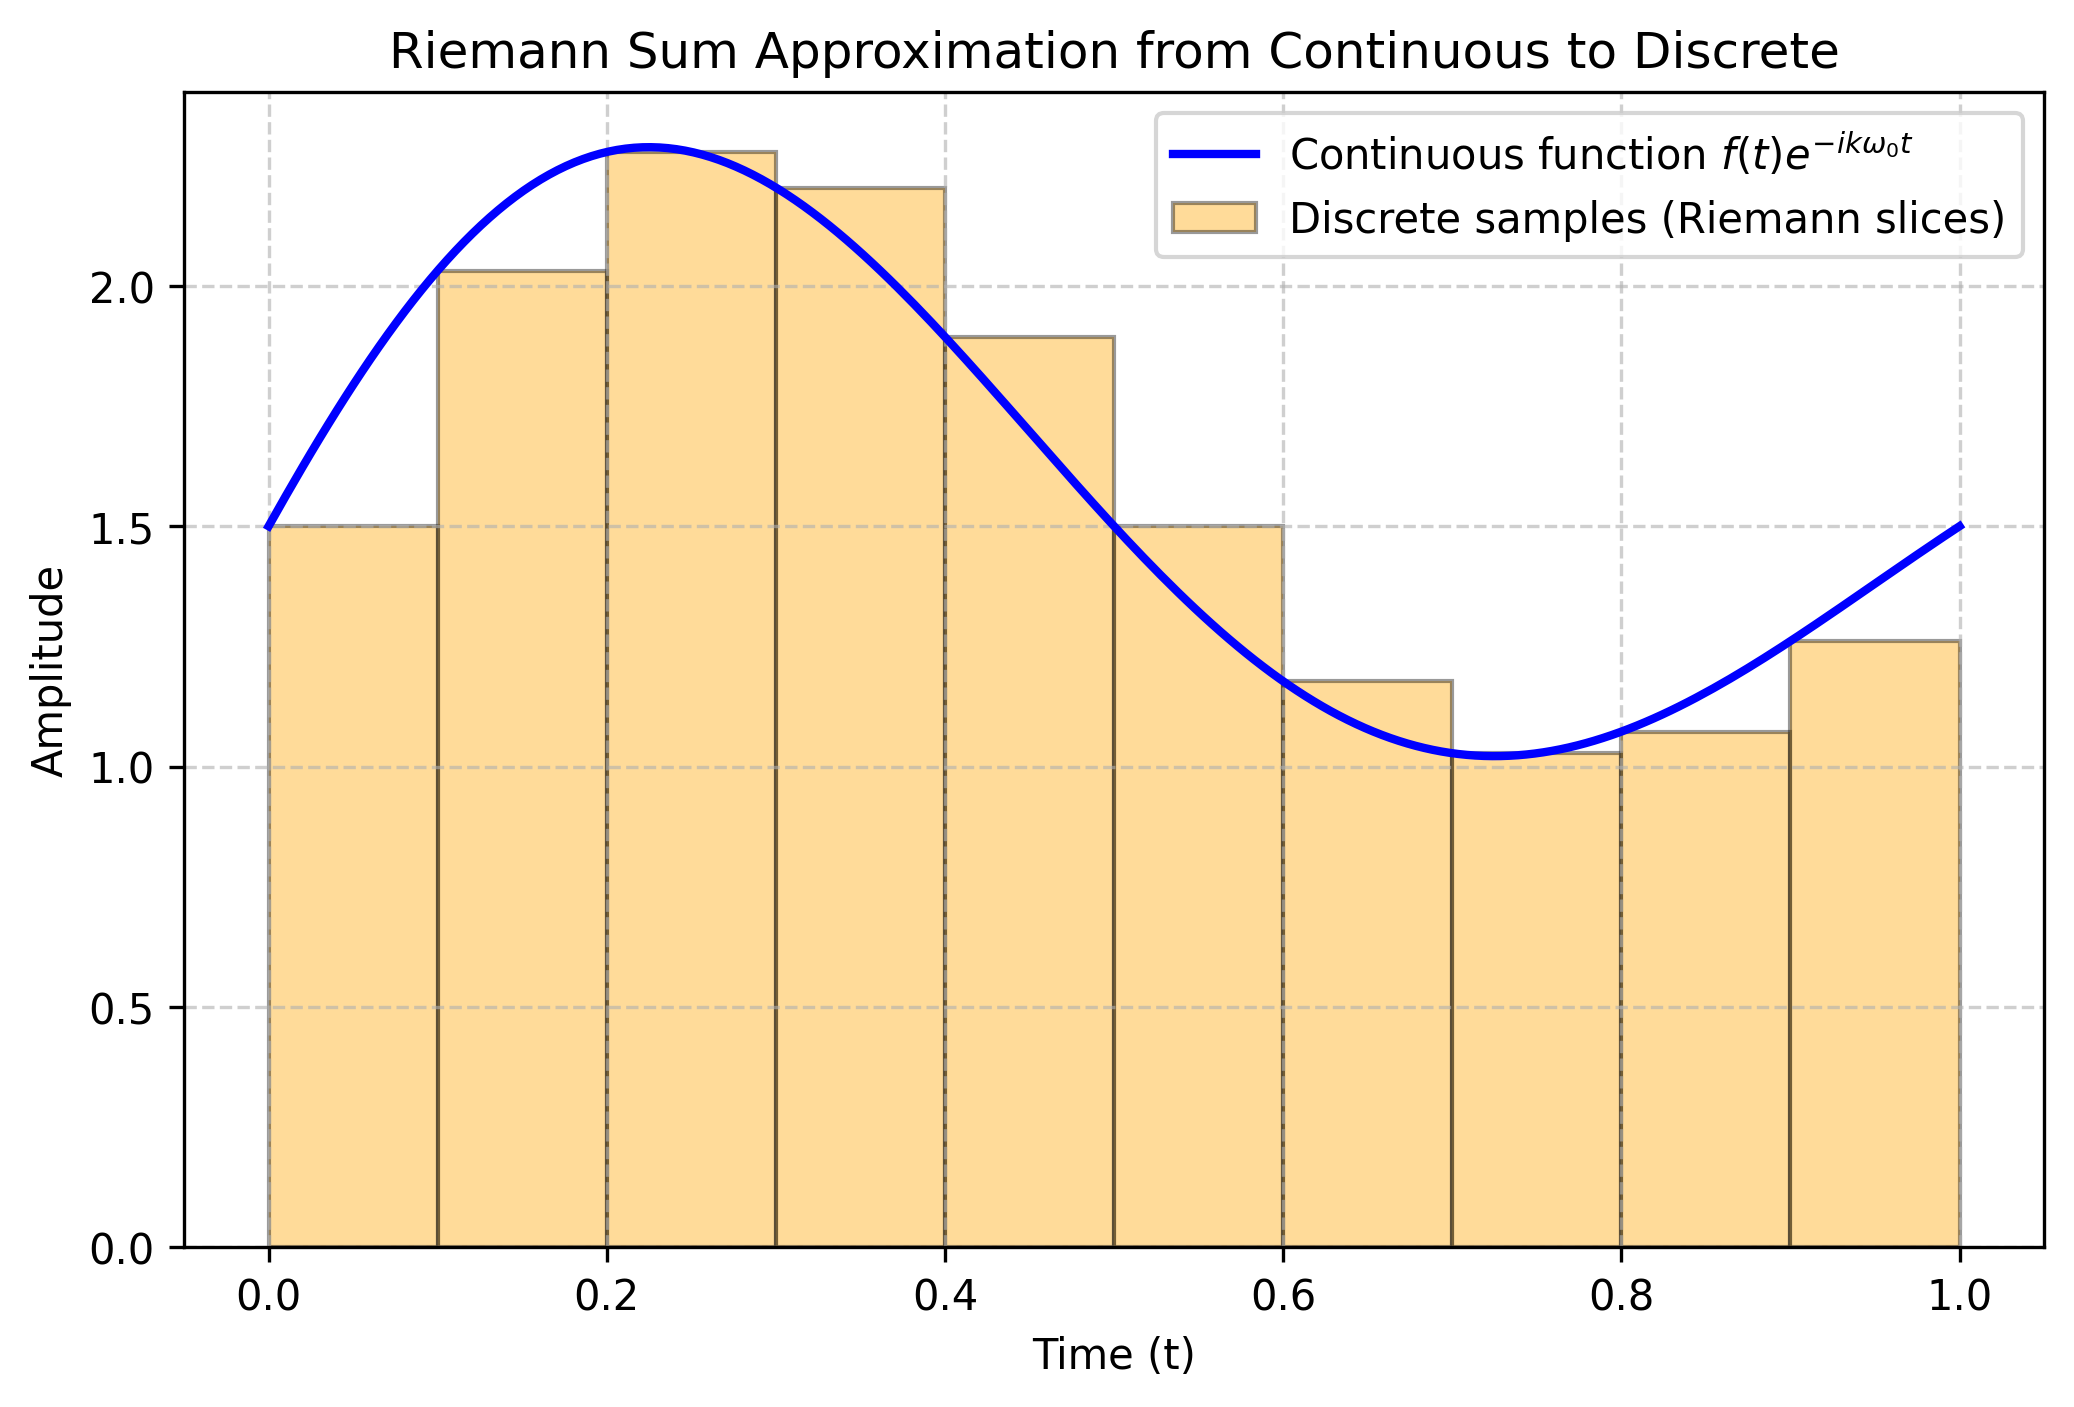
\includegraphics[width=0.7\textwidth]{riemann_sum.png} 
    \caption{A visual representation of the Riemann sum approximation, where the continuous area under the signal $f(t)$ is approximated by discrete rectangular slices of width $\Delta t$.}
    \label{fig:riemann_sum}
\end{figure}

\begin{equation}
    c_k = \frac{1}{T}\int_{0}^{T} f(t)\, e^{-i k \omega_0 t}\, dt.
    \label{eq:ck_cont_redef}
\end{equation}

This geometric approximation involves a formal mapping from the continuous domain to the discrete domain:
\begin{itemize}
    \item A continuous signal $f(t)$ is sampled at $N$ uniform points, which geometrically dictates the height of each rectangle in our sum, yielding a sequence of values $x_n = f(t_n)$.
    \item The continuous time variable $t$ is replaced by discrete time points $t_n = n\Delta t$, representing the left edge of the $n$-th rectangle, for $n = 0, 1, \dots, N-1$.
    \item The infinitesimal differential $dt$ (the continuous base of the integral) is replaced by the finite width of each rectangle, the sampling period $\Delta t = T/N$.
    \item The integral $\int$ is replaced by a sum $\sum$ over the areas of the $N$ discrete samples.
\end{itemize}

Applying these substitutions to \eqref{eq:ck_cont_redef}, with $\omega_0=2\pi/T$:
\begin{align}
    c_k 
    &\approx \frac{1}{T}\sum_{n=0}^{N-1} f(t_n) \cdot e^{-i k (2\pi/T) (n\Delta t)} \cdot \Delta t \nonumber \\
    &= \frac{1}{T}\sum_{n=0}^{N-1} x_n \cdot e^{-i 2\pi k n (T/N) / T} \cdot (T/N) \nonumber \\
    &= \frac{1}{N}\sum_{n=0}^{N-1} x_n \, e^{-i 2\pi k n / N}.
    \label{eq:ck_discrete}
\end{align}
Getting this discrete formula to match the continuous theory was an initial roadblock for me. I spent hours staring at the 1/T term in the continuous integral, wondering how the algorithm was supposed to handle a continuous time period when all I had were discrete data points. It finally clicked when I drew out the rectangles. The base of each rectangle, delta t, is simply the total time T divided by the total number of samples N. When I substituted that ratio into the equation, the time variables completely canceled out, leaving just the 1/N scaling factor. Seeing that algebraic cancellation happen on paper was incredibly satisfying. This final expression forms the theoretical link between the continuous Fourier coefficient and the DFT. I found this step surprisingly satisfying, because it showed that the DFT wasn’t some black-box algorithm; it’s literally the continuous integral cut into slices, which made me trust my later code more when I wrote it based on this principle.

\paragraph{Implications of Discretization.}
This conversion from a continuous integral to a discrete sum imposes two fundamental constraints on the analysis.
\begin{itemize}
    \item \textbf{Frequency Resolution ($\Delta f$):} The DFT calculates the spectrum at discrete frequency "bins". The spacing between these bins, or the smallest frequency it can resolve, is the frequency resolution, $\Delta f = 1/T$, where $T$ is the total duration of the sample window. For my chosen window of $T=0.05$\,s, the resolution is $\Delta f = 1/0.05 = 20$\,Hz. This means my analysis can only distinguish frequencies in integer multiples of 20\,Hz.
    \item \textbf{Nyquist Frequency ($f_{Nyquist}$):} When converting a continuous signal into discrete samples, there is a strict limit on the maximum frequency that can be accurately measured. As illustrated in Figure \ref{fig:aliasing}, if a wave oscillates too rapidly between sample points, the discrete data will misinterpret it as a lower frequency—an error known as aliasing. 
    
    \begin{figure}[H]
        \centering
        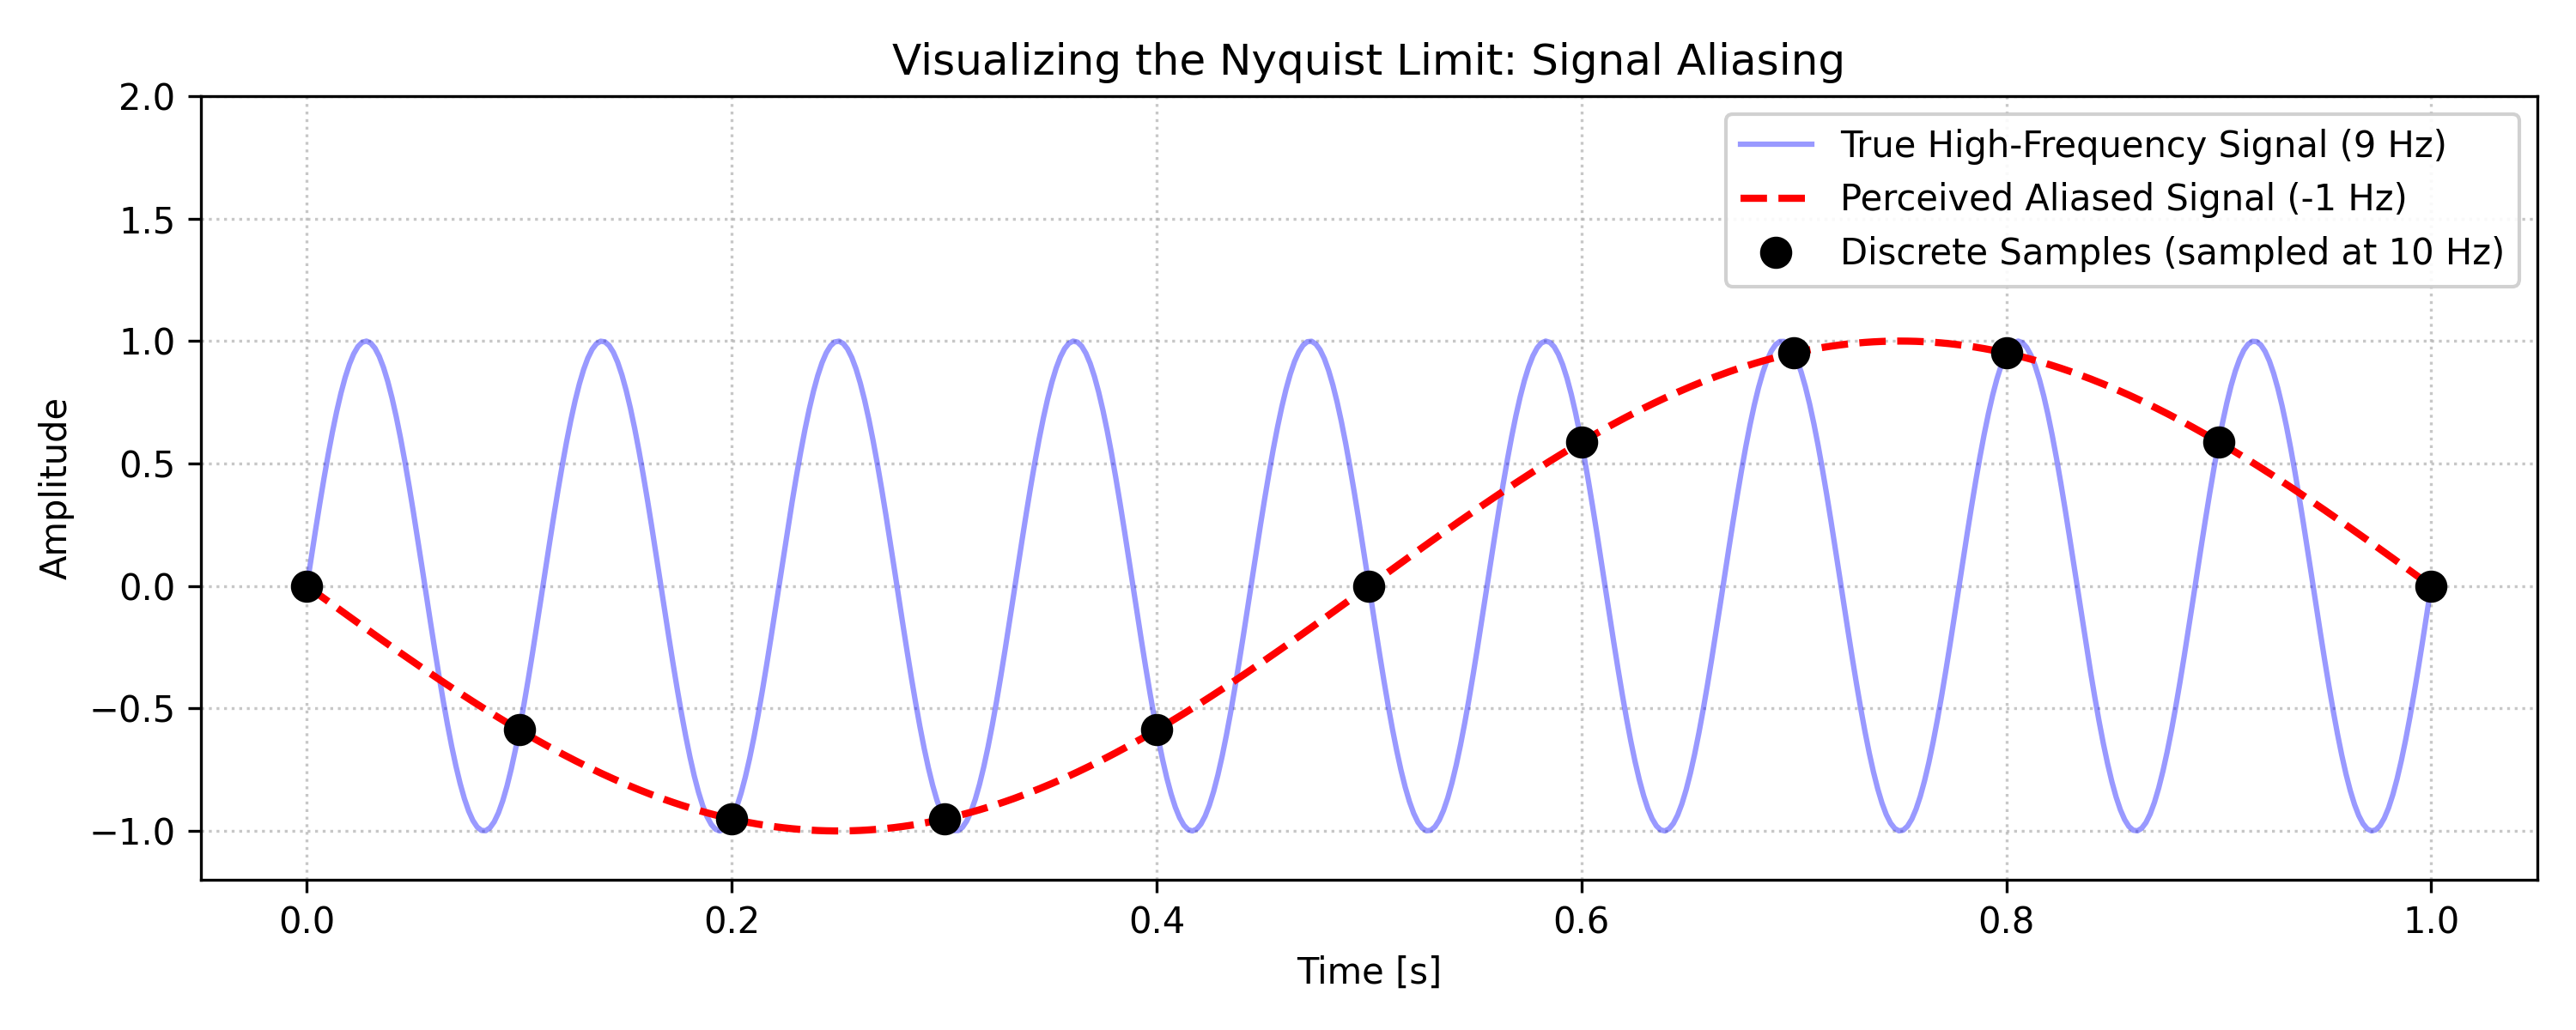
\includegraphics[width=0.8\textwidth]{aliasing_diagram.png} 
        \caption{A visual demonstration of aliasing. The high-frequency actual signal (solid blue) is sampled too sparsely (black dots). When reconstructed, these sample points erroneously form a low-frequency alias signal (dashed red), demonstrating why the sampling rate must exceed the Nyquist limit.}
        \label{fig:aliasing}
    \end{figure}

    To prevent this, the Nyquist-Shannon sampling theorem dictates that the sampling rate ($f_s$) must be strictly greater than twice the highest frequency present in the signal \cite{stein2003fourier}. The maximum unambiguous frequency is the Nyquist frequency, calculated as $f_{Nyquist} = f_s/2$. For my audio data, sampled at the standard CD rate of $f_s = 44100$\,Hz, this upper limit is $22050$\,Hz. Since this is well above the upper limit of human hearing (and the mechanical limits of a guitar string), I can be mathematically certain that no high-frequency harmonics are "folding back" and corrupting my lower-frequency results.
\end{itemize}

\paragraph{Definition of the DFT.}
The discrete approximation for $c_k$ motivates the definition of the \emph{Discrete Fourier Transform}. 
For a sequence of $N$ samples $\{x_0,x_1,\dots,x_{N-1}\}$, the DFT produces coefficients
\begin{equation}
    X_k = \sum_{n=0}^{N-1} x_n\, e^{-i 2\pi k n / N}, 
    \qquad k = 0,1,\dots,N-1.
    \label{eq:dft}
\end{equation}
Comparing \eqref{eq:ck_discrete} and \eqref{eq:dft}, we see that
\begin{equation}
    c_k \approx \frac{1}{N}X_k,
\end{equation}
so the DFT coefficients $X_k$ are simply scaled versions of the continuous Fourier coefficients.

\paragraph{Sample Calculation of the DFT.}
To demonstrate the mechanics of Equation \eqref{eq:dft}, consider a simplified "toy" signal consisting of $N=4$ samples representing a basic oscillation: $x_n = \{1, 0, -1, 0\}$. I will manually calculate two coefficients: $X_1$ (to test for the presence of a matching frequency) and $X_0$ (to test for a constant DC offset). 

First, calculating $X_1$ ($k=1$) using the DFT formula:
\begin{equation*}
    X_1 = \sum_{n=0}^{3} x_n e^{-i 2\pi (1) n / 4} = \sum_{n=0}^{3} x_n e^{-i \pi n / 2}
\end{equation*}

This generates four exponential terms as $n$ changes. As visually illustrated in Figure \ref{fig:unit_circle_roots}, these values lie on a circle of radius 1 in the complex plane, separated by $90^\circ$ ($\pi/2$ radians). This diagram provides the geometric proof for converting these exponential terms into simple real and imaginary numbers. Expanding the summation for each sample $n$:
\begin{equation}
    X_1 = x_0 \underbrace{e^0}_{1} + x_1 \underbrace{e^{-i \pi / 2}}_{-i} + x_2 \underbrace{e^{-i \pi}}_{-1} + x_3 \underbrace{e^{-i 3\pi / 2}}_{i}
    \label{eq:expanded_sum}
\end{equation}

\begin{figure}[H]
    \centering
    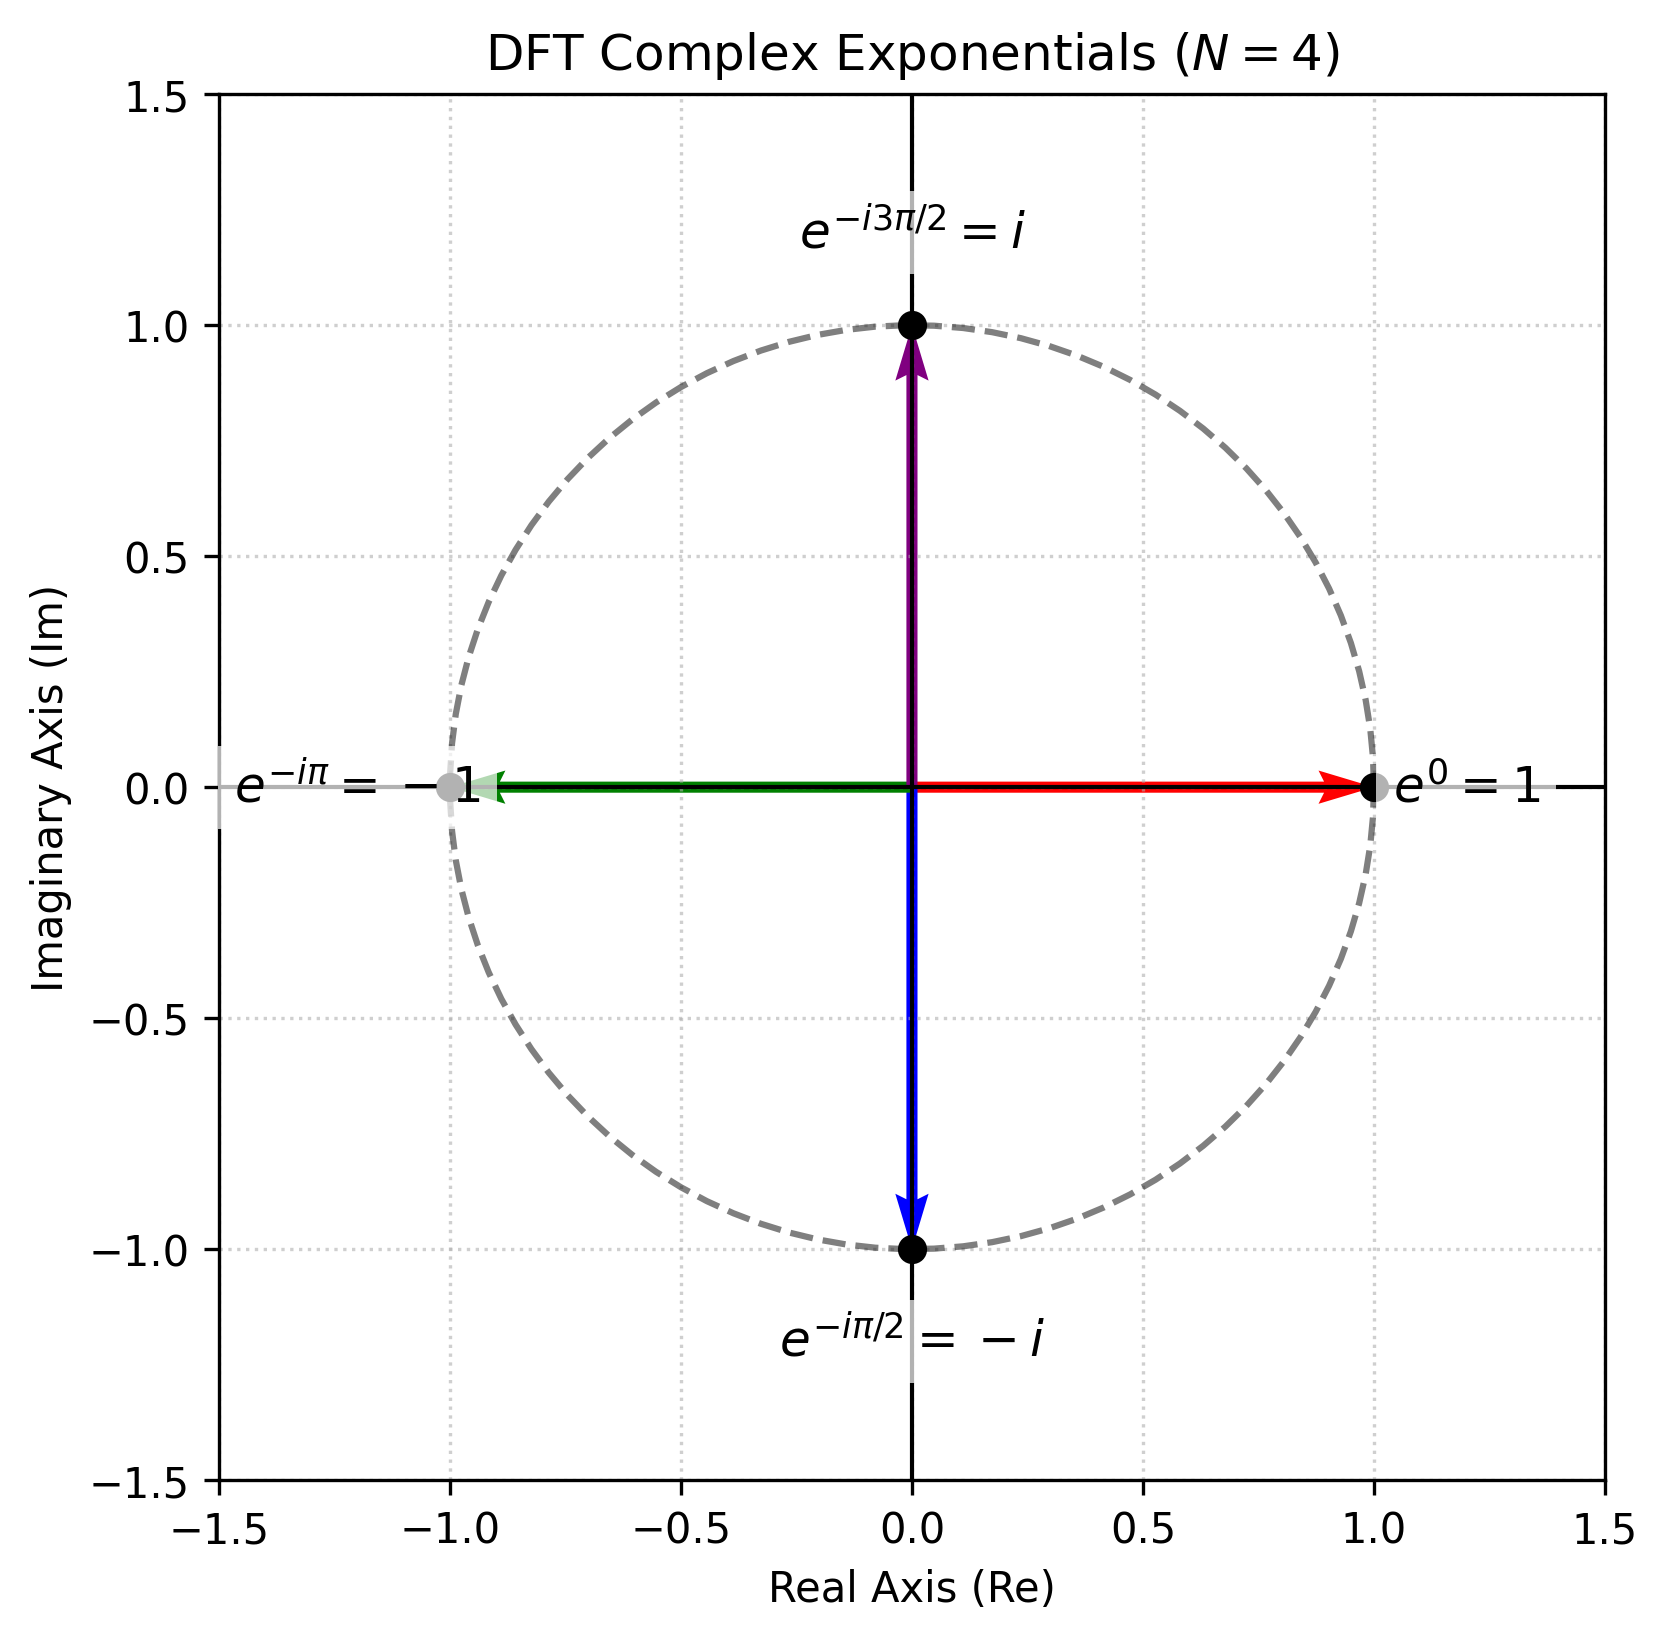
\includegraphics[width=0.45\textwidth]{unit_circle_roots.png} 
    \caption{Argand Diagram of the complex exponential terms used in the 4-point sample calculation, showing how they rotate around the unit circle to specific positions.}
    \label{fig:unit_circle_roots}
\end{figure}

The conversion of these complex exponential terms to simple integers is mathematically verified using Euler's identity ($e^{-i\theta} = \cos\theta - i\sin\theta$). Substituting the values of the signal samples $\{x_0=1, x_1=0, x_2=-1, x_3=0\}$ into \eqref{eq:expanded_sum} gives the final sum for $X_1$:
\begin{align*}
    X_1 &= (1)(1) + (0)(-i) + (-1)(-1) + (0)(i) \\
    X_1 &= 1 + 0 + 1 + 0 = 2.
\end{align*}

Next, calculating $X_0$ ($k=0$):
\begin{equation*}
    X_0 = \sum_{n=0}^{3} x_n e^{-i 2\pi (0) n / 4} = \sum_{n=0}^{3} x_n e^0
\end{equation*}
\begin{align*}
    X_0 &= (1)(1) + (0)(1) + (-1)(1) + (0)(1) \\
    X_0 &= 1 + 0 - 1 + 0 = 0.
\end{align*}

This sample calculation proves how the DFT isolates specific frequencies. For $X_1$, the complex exponentials constructively interfere with the data, yielding a magnitude of 2 because the signal's frequency matches the basis function. For $X_0$, the terms destructively interfere to exactly $0$. Crucially, this calculated magnitude of 2 directly corresponds to the height of the peaks plotted on the $y$-axis of my actual frequency spectrum (such as in Figure \ref{fig:spectrum}). By iterating this exact mathematical process across all 2205 samples and all frequency bins, the Python script in Appendix A constructs the complete graph of the guitar note.

\paragraph{The inverse DFT.}
The ability to perfectly reconstruct the original signal $\{x_n\}$ from its coefficients $\{X_k\}$ via the \emph{inverse DFT} relies on the orthogonality of the discrete exponential basis functions. This property is the discrete analogue of the one proven for the continuous case.

\textbf{Proof of Discrete Orthogonality:} We must show $\sum_{n=0}^{N-1} e^{i2\pi(k-j)n/N} = N$ for $k=j$ and $0$ for $k \ne j$. Let $m=k-j$ and the ratio $r = e^{i2\pi m/N}$. The sum is a finite geometric series $\sum_{n=0}^{N-1} r^n$.
\begin{itemize}
    \item For $k=j$, $m=0$ and $r=e^0=1$. The sum is $\sum_{n=0}^{N-1} 1 = N$.
    \item For $k \neq j$, $r \neq 1$. The sum is $\frac{r^N-1}{r-1}$. The numerator $r^N = (e^{i2\pi m/N})^N = e^{i2\pi m} = 1$, since $m$ is a non-zero integer. Thus the sum is $\frac{1-1}{r-1} = 0$.
\end{itemize}
This orthogonality ensures the inverse transformation is exact:
\begin{equation}
    x_n = \frac{1}{N}\sum_{k=0}^{N-1} X_k\, e^{i 2\pi k n / N}, 
    \qquad n = 0,1,\dots,N-1.
    \label{eq:idft}
\end{equation}
This algebraic inverse ensures that the transformation between $\{x_n\}$ and $\{X_k\}$ is lossless, 
limited only by floating-point precision when implemented on a computer.

\paragraph{Frequency interpretation.}
Each index $k$ corresponds to the physical frequency
\begin{equation}
    f_k = \frac{k}{N} f_s,
    \label{eq:freq_map}
\end{equation}
where $f_s = 1/\Delta t$ is the sampling rate. The highest resolvable frequency is $f_s/2$, known as the 
\emph{Nyquist frequency}. For real-valued signals $x_n$, the spectrum is conjugate-symmetric 
($X_{N-k} = \overline{X_k}$), so it is customary to plot only the nonnegative frequencies 
$0 \leq f \leq f_s/2$.

\paragraph{Interpretation in this investigation.}
The DFT provides the exact computational analogue of the continuous Fourier series. 
Instead of evaluating integrals, I apply \eqref{eq:dft} to the sampled guitar waveform. 
The resulting coefficients $X_k$ encode both the amplitude and phase of the sinusoidal components 
that make up the note. By using \eqref{eq:idft}, I can reconstruct the waveform directly from these coefficients, 
providing a rigorous way to check whether the sinusoidal decomposition captures the original signal exactly.

\begin{figure}[H]
    \centering
    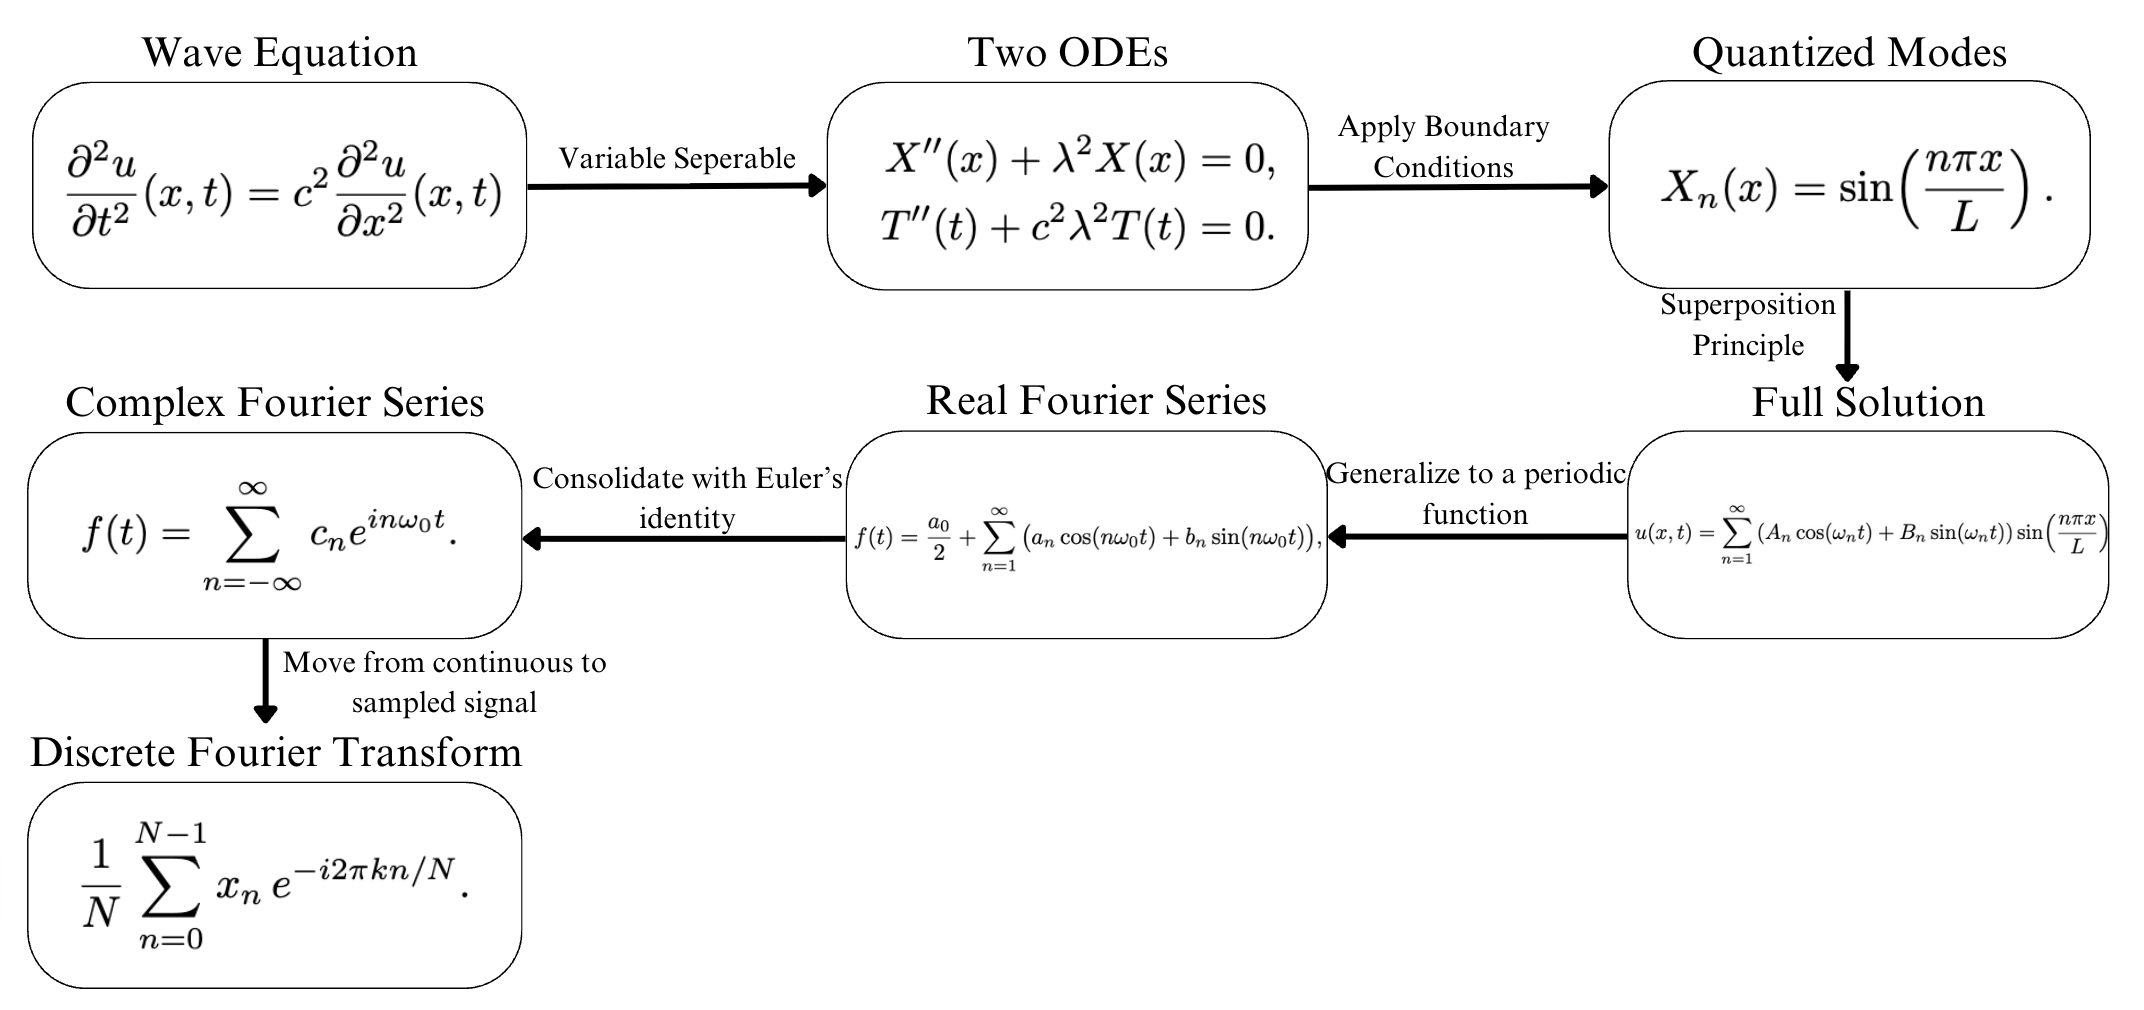
\includegraphics[width=\textwidth]{flowchart.png}
    \caption{A flowchart illustrating the logical progression of the theoretical framework, from the physical model of the wave equation to the final computational tool of the Discrete Fourier Transform.}
    \label{fig:theory_flowchart}
\end{figure}

% --- METHODOLOGY ---
\section{Methodology}

\subsection{Data Acquisition and Preparation}
I initially tried recording my own acoustic guitar using my phone microphone. When I ran that data through my initial code, the resulting spectrum was a chaotic mess of random frequencies instead of clean peaks. After days of confusion, I realized the phone software was automatically applying noise cancellation and audio compression. These digital filters were artificially destroying the natural physical harmonics of the string. I had to pivot to find a pure, uncompressed audio source. For the analysis, I needed a perfectly clean sound wave. I decided to use a pre-recorded sample from the University of Iowa music database instead of fighting with my own recording setup \cite{iowa}. This way, I avoided room acoustics or microscopic mic distortions ruining the data, allowing me to focus entirely on the pure mathematics of the sound. The file was a mono wav recording sampled at 44100 Hz.

The raw audio file contains several notes. To get a good sample for Fourier analysis, which works on periodic functions, I first had to find and isolate a single note (Figure \ref{fig:full_waveform} and \ref{fig:note_closeup}).

\begin{figure}[H]
    \centering
    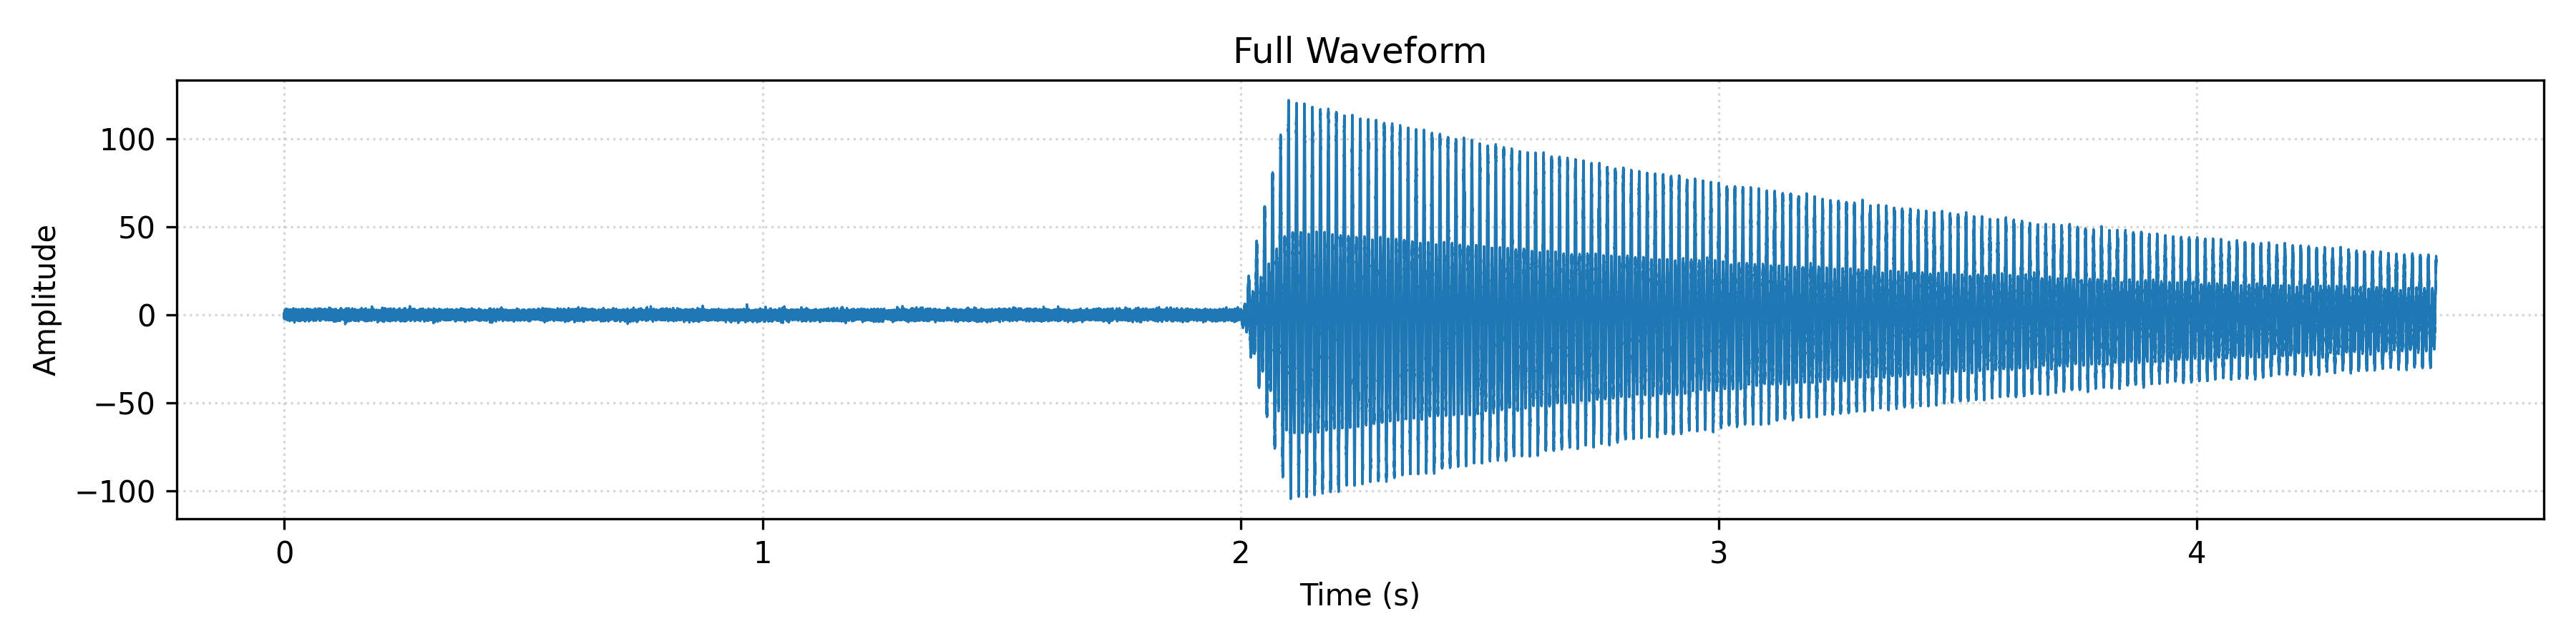
\includegraphics[width=\textwidth]{full_waveform.png}
    \caption{The full waveform of the audio file, showing multiple distinct note events.}
    \label{fig:full_waveform}
\end{figure}

\begin{figure}[H]
    \centering
    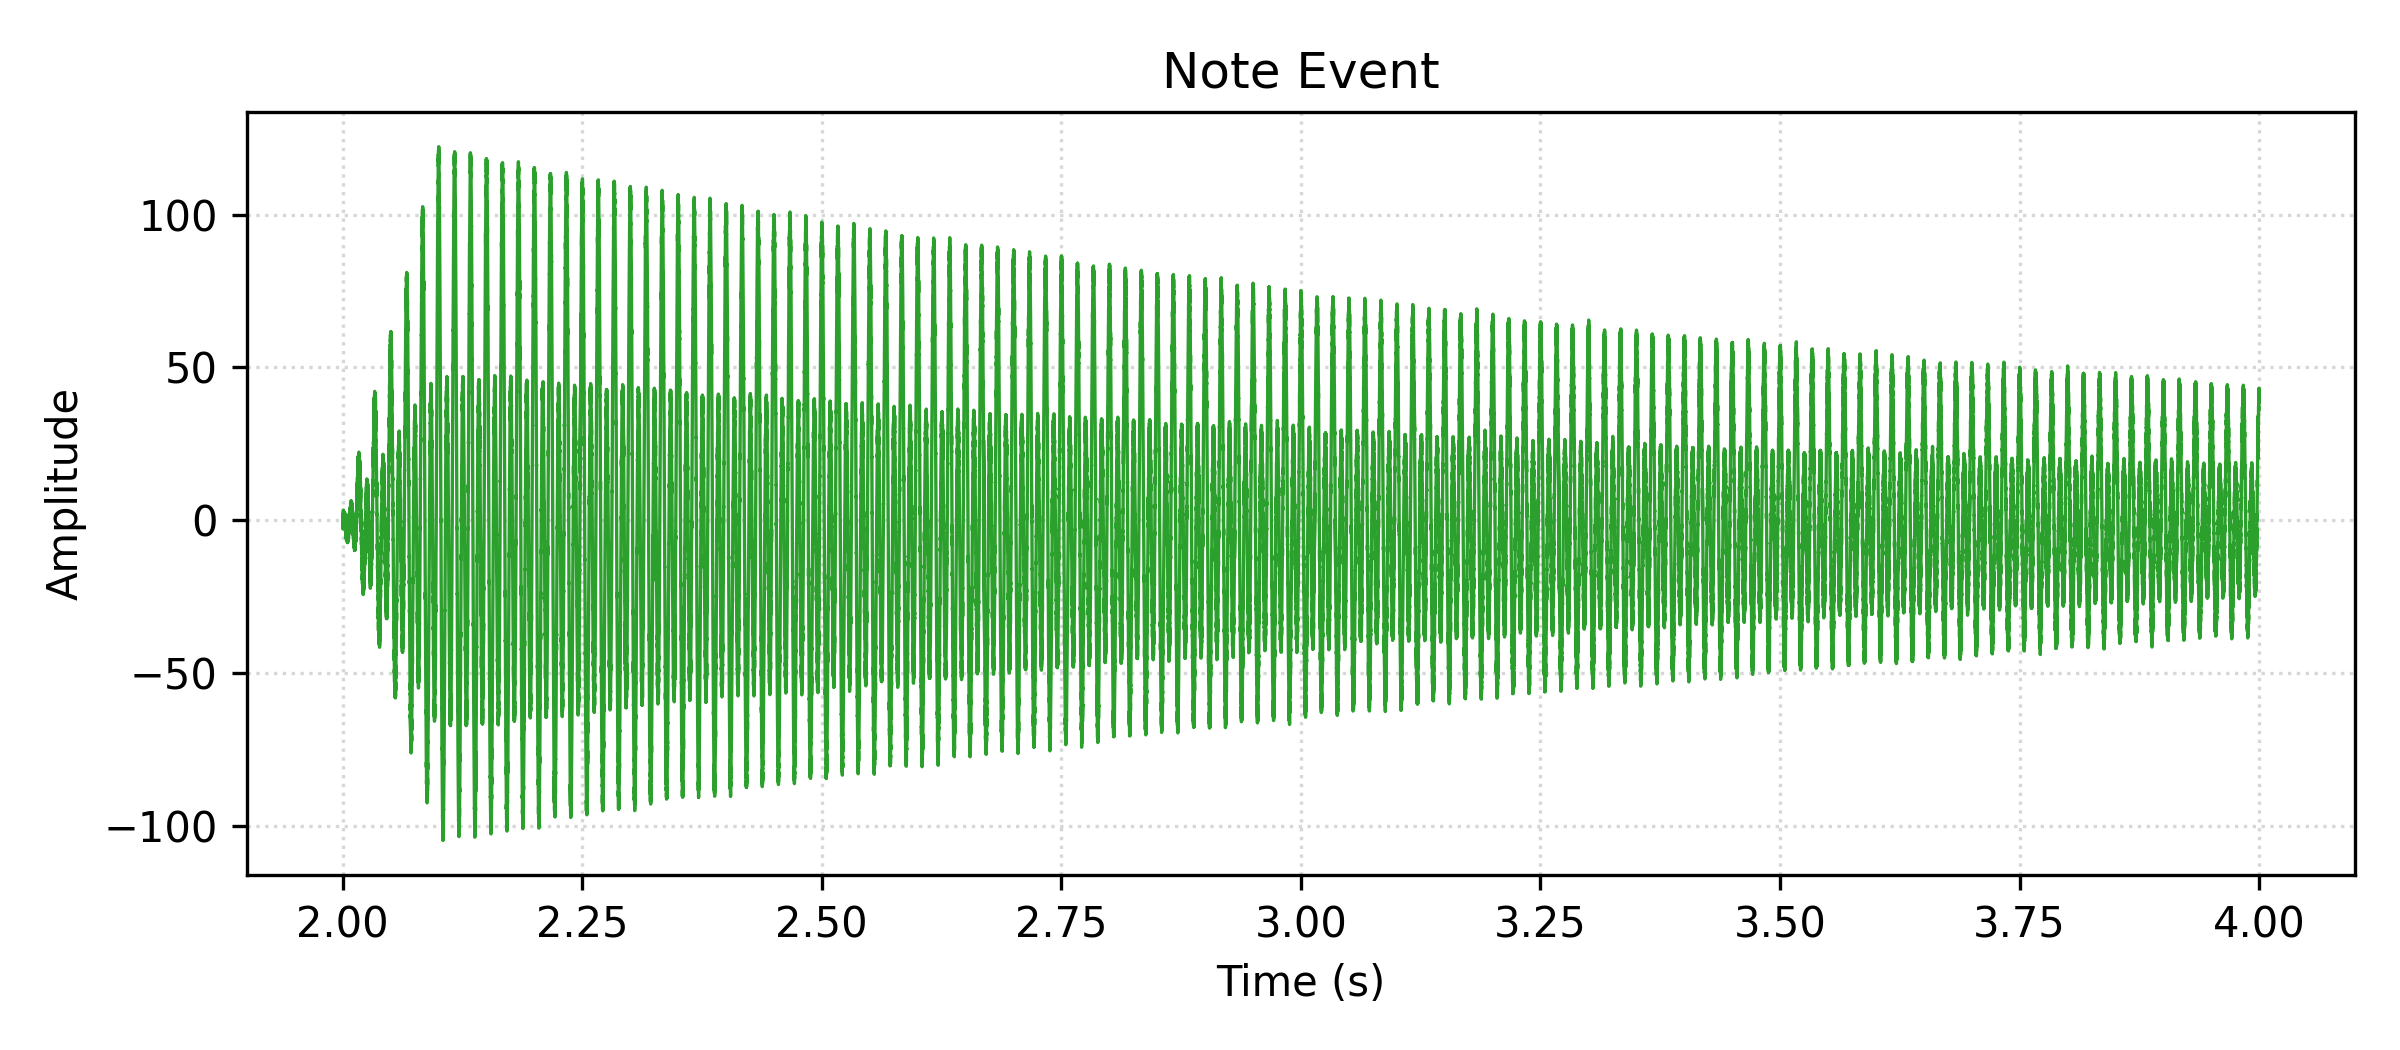
\includegraphics[width=\textwidth]{note_closeup.png}
    \caption{A close-up view of a single note event, showing the initial attack and subsequent decay.}
    \label{fig:note_closeup}
\end{figure}

From that single note, I cut out a small, stable segment of 0.05 seconds from the middle, avoiding the transient irregularities during the attack and decay phases of the note. This duration was deliberately chosen to yield a frequency resolution of $\Delta f = 1/T = 1/0.05 = 20$\,Hz. This choice also highlights a fundamental concept in signal processing analogous to the uncertainty principle: there is an inherent trade-off between time resolution and frequency resolution. Our time window of $\Delta t=0.05$\,s fixes our frequency resolution at $\Delta f=1/\Delta t=20$\,Hz. Achieving a finer frequency resolution would necessarily require analyzing a longer, and potentially less stable, time segment. This final slice (Figure \ref{fig:isolated_segment}) is the function, $f(t)$, that I analyze in the rest of the IA.

\begin{figure}[H]
    \centering
    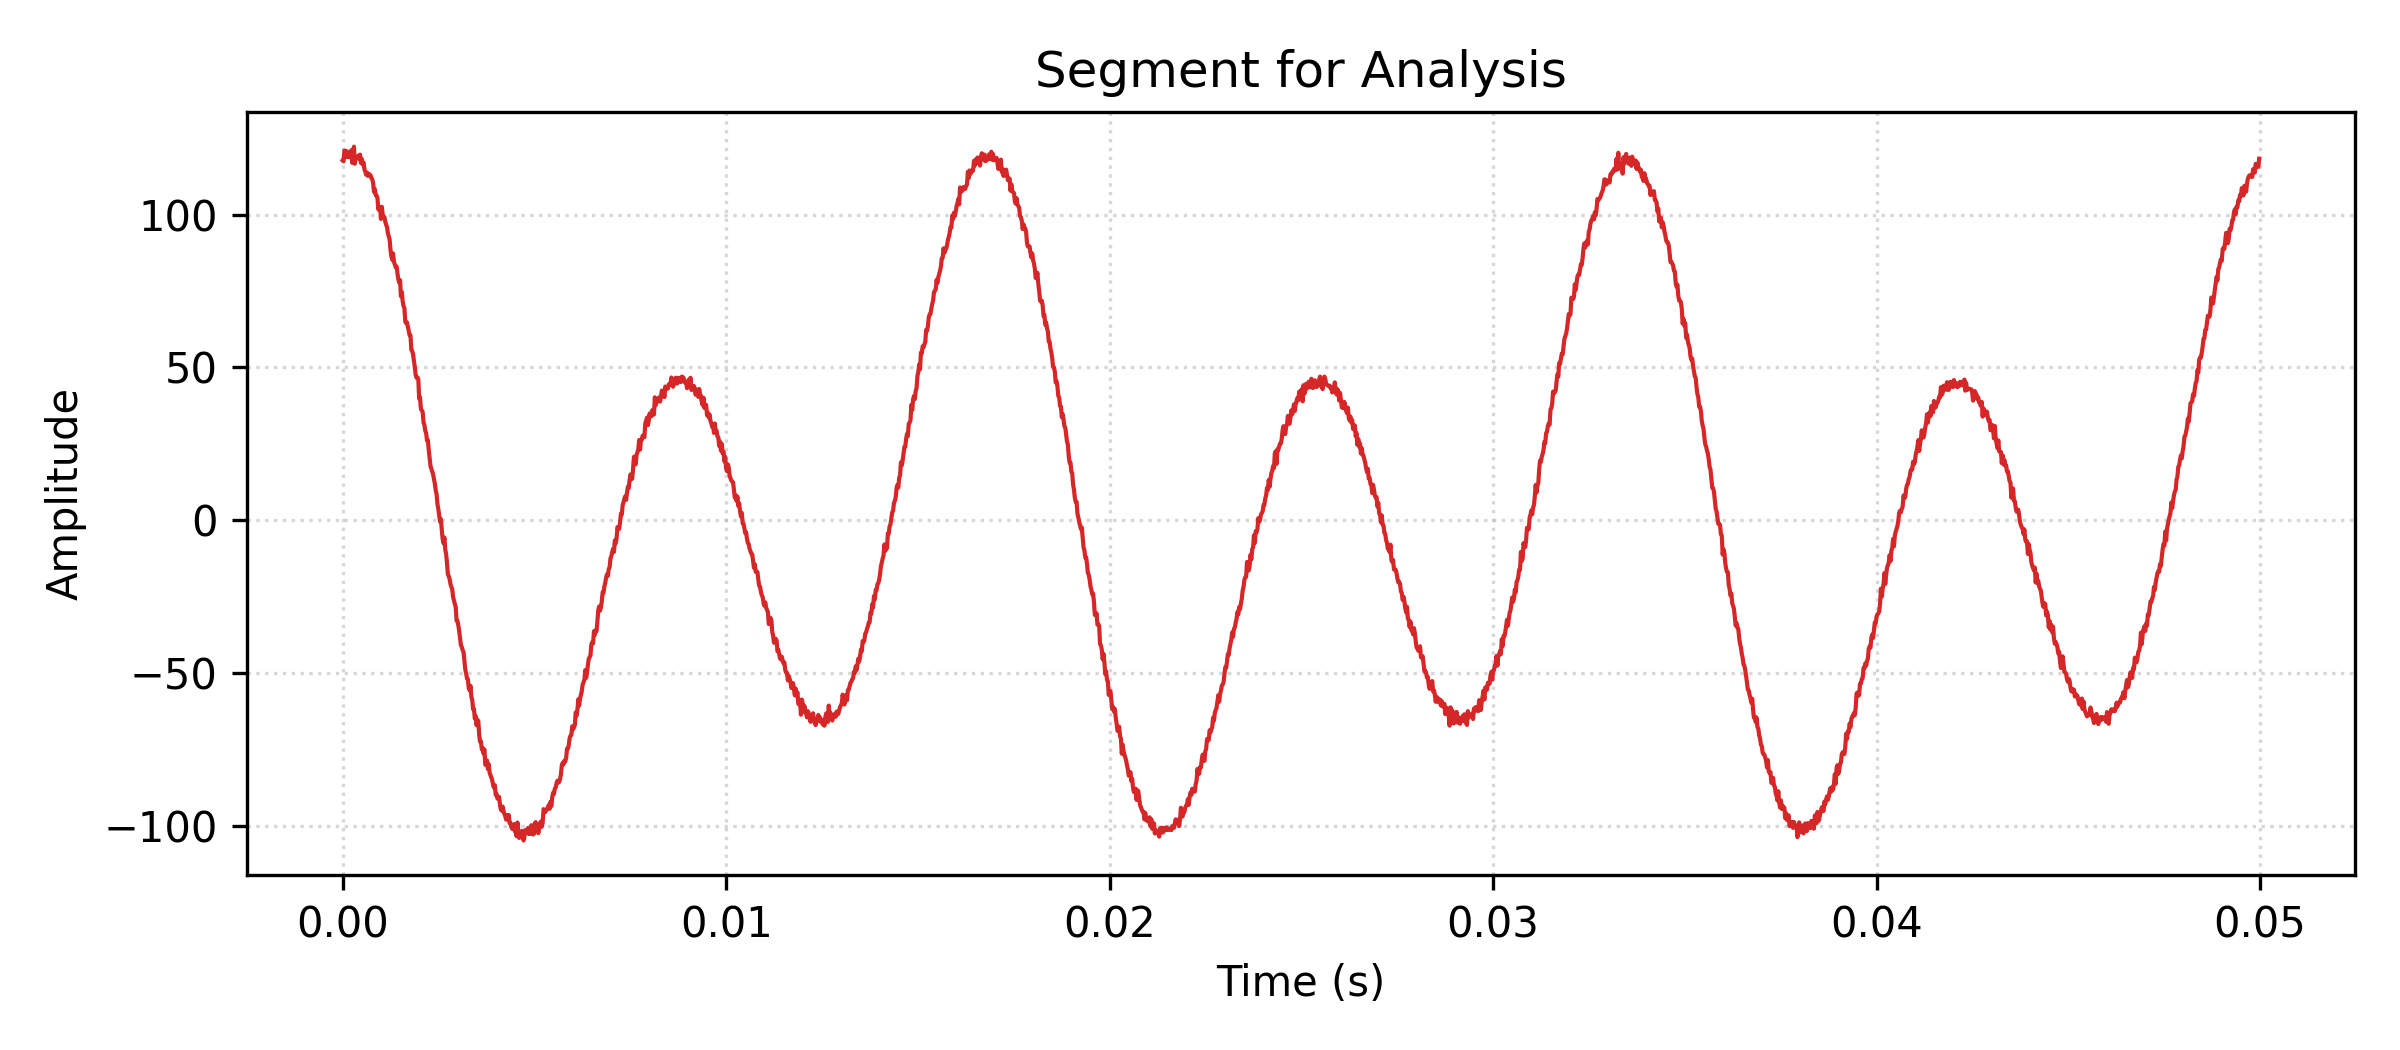
\includegraphics[width=\textwidth]{isolated_segment.png}
    \caption{The isolated 0.05s segment used for Fourier analysis.}
    \label{fig:isolated_segment}
\end{figure}

\subsection{Computational Analysis Strategy}
The entire computational process, including the application of the DFT and the generation of all subsequent plots and calculations, was implemented programmatically using Python. The full code script is provided in Appendix A. The analysis followed three main steps:
\begin{enumerate}
    \item \textbf{Deconstruction:} The manual DFT is applied to the isolated waveform segment to calculate the set of complex coefficients $X_k$.
    \item \textbf{Analysis:} The magnitudes of these coefficients are plotted against their corresponding frequencies to generate a frequency spectrum, revealing the harmonic structure of the note.
    \item \textbf{Reconstruction:} The Inverse DFT is used to synthesize a new waveform from the calculated coefficients, allowing for a direct visual and quantitative comparison against the original signal.
\end{enumerate}

% --- RESULTS AND ANALYSIS ---
\section{Results and Analysis}

\subsection{The Frequency Spectrum: Deconstructing the Waveform}
Applying the DFT to my waveform segment gave me the frequency spectrum in Figure \ref{fig:spectrum}. This plot shows the strength of each frequency that makes up the sound, effectively translating the waveform into a harmonic fingerprint.

\begin{figure}[H]
    \centering
    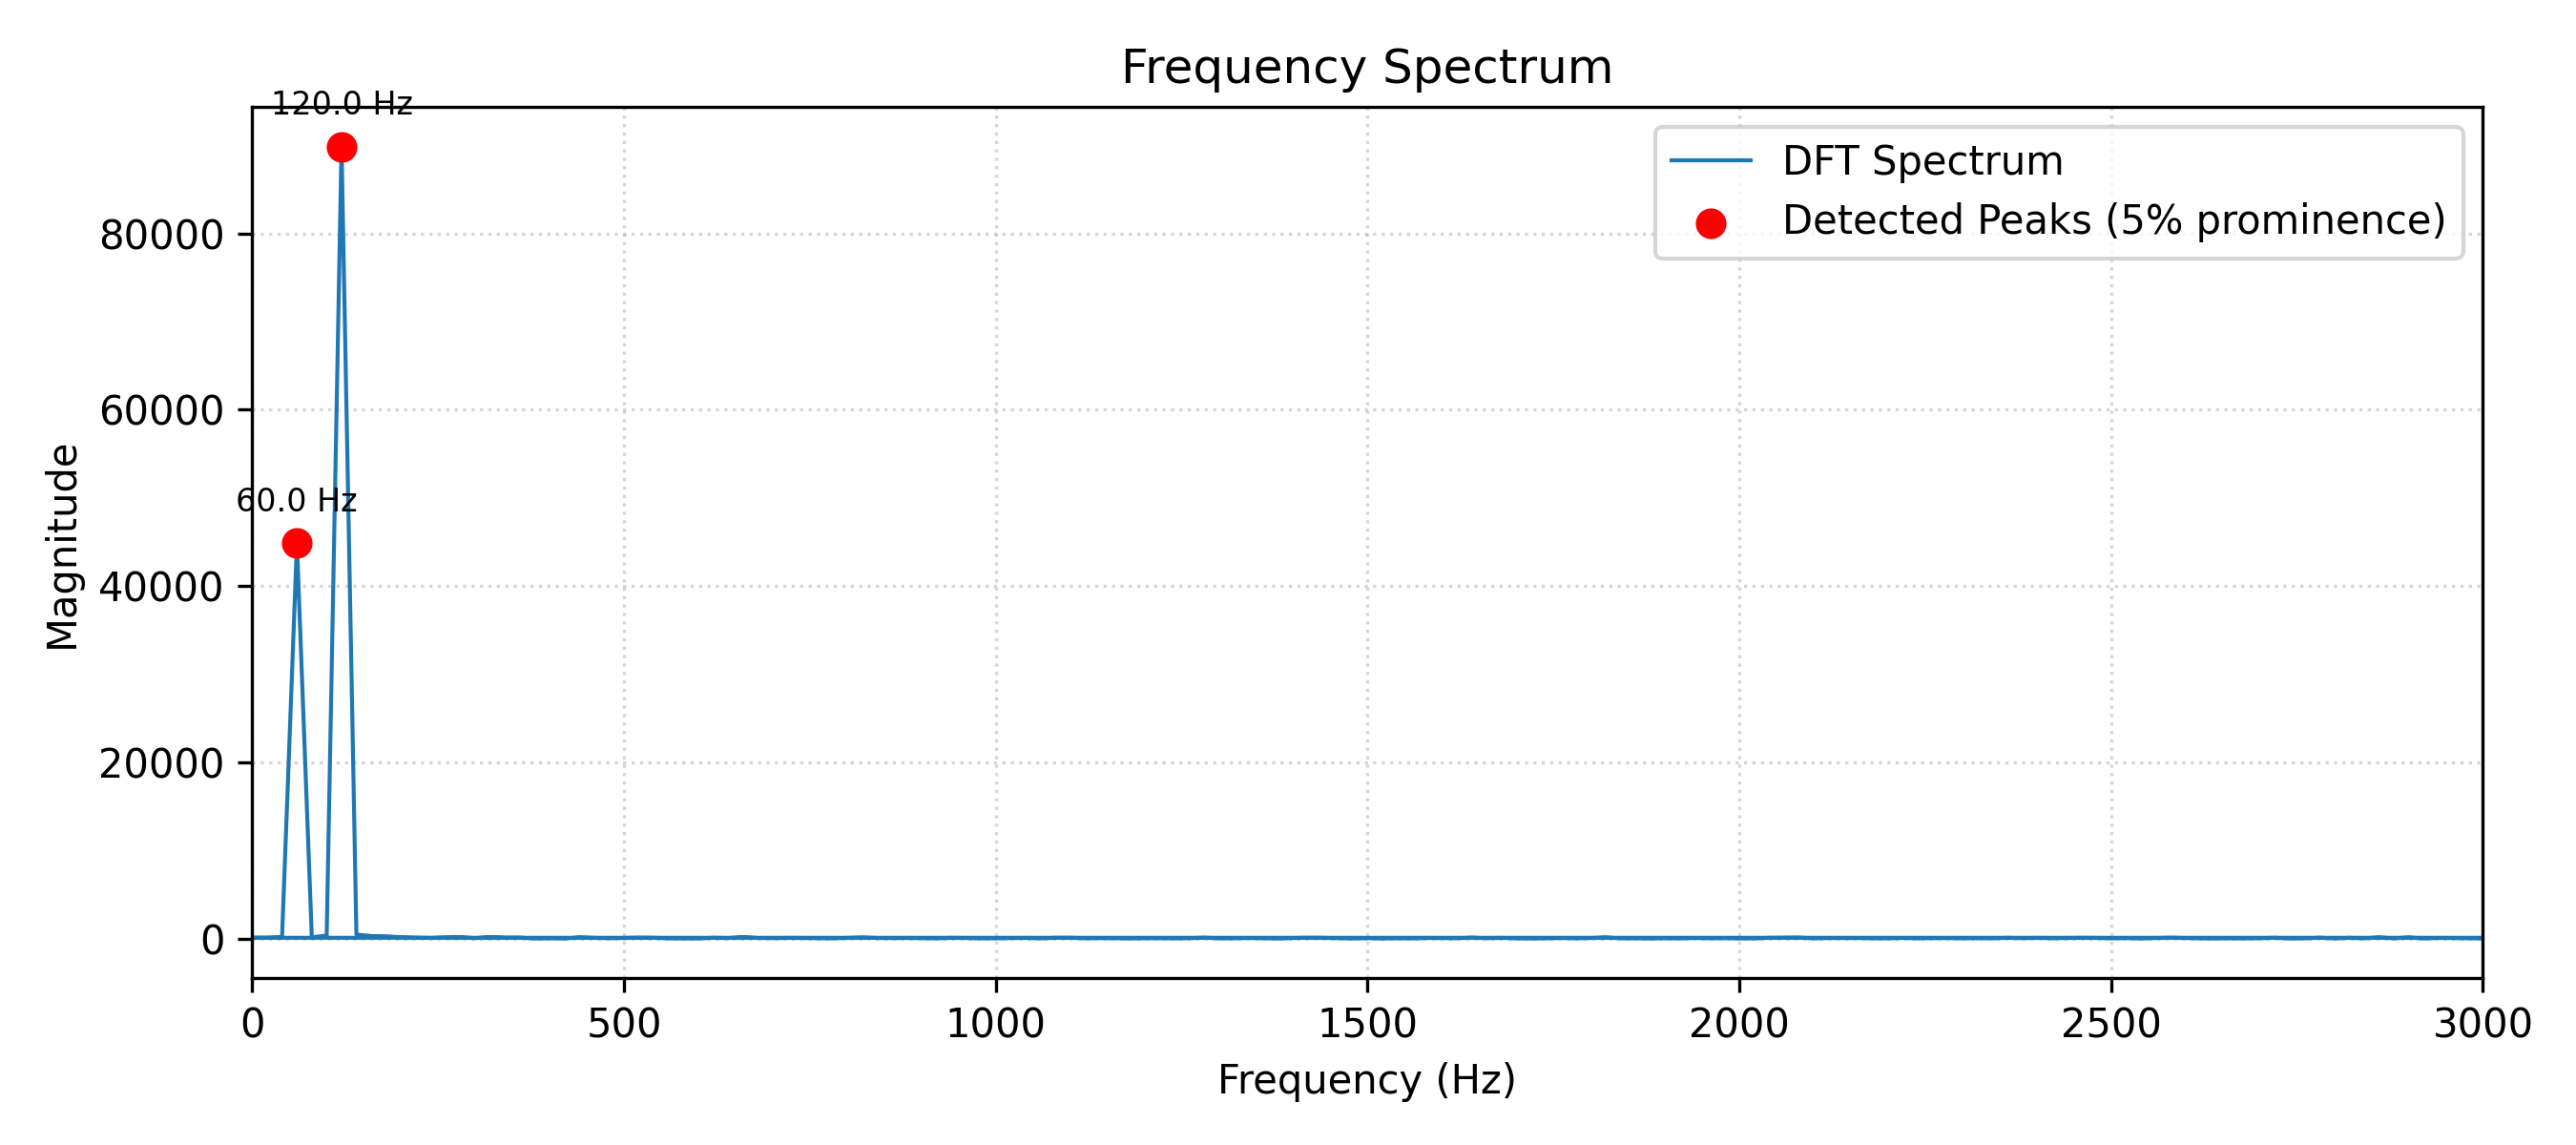
\includegraphics[width=\textwidth]{spectrum.png}
    \caption{The frequency spectrum of the guitar note segment. The x-axis is frequency in Hz, and the y-axis is the magnitude of the complex coefficient. Detected peaks are marked in red. No further significant peaks were found beyond 120 Hz.}
    \label{fig:spectrum}
\end{figure}

Instead of just eyeballing the graph, I used a peak-finding algorithm to get objective measurements. Mathematically, the algorithm identifies a frequency bin $k$ as a local maximum (a peak) if its magnitude $M_k$ is strictly greater than its immediate neighbors: $M_{k-1} < M_k > M_{k+1}$. 

In my very first spectral plot, I was confused to see tiny spikes appearing at extremely high frequencies. I originally hypothesized these were exotic guitar overtones. However, after calculating the Nyquist frequency, I recognized they were just mathematical artifacts and background static from the recording equipment. I learned that real-world data is never perfectly clean. To filter out background noise, I set a prominence threshold to 5 percent of the magnitude of the largest peak. The results are in Table \ref{tab:harmonics}.

\begin{table}[H]
    \centering
    \caption{Algorithmically Detected Harmonic Frequencies and Magnitudes}
    \begin{tabular}{@{}ccc@{}}
        \toprule
        Harmonic & Frequency (Hz) & Magnitude (Arbitrary Units) \\ \midrule
        Fundamental ($f_0$) & 60.00          & 45391.50  \\
        1st Overtone (2$f_0$) & 120.00         & 91096.02  \\ 
        \bottomrule
    \end{tabular}
    \label{tab:harmonics}
\end{table}

Only two harmonics were detected above the threshold. Higher harmonics, while theoretically possible, were below this detection cut-off, indicating that this note’s timbre is dominated by the fundamental and first overtone. The detected peaks at 60.00\,Hz and 120.00\,Hz align perfectly with the 3rd ($k=3$) and 6th ($k=6$) frequency bins of the DFT, as predicted by the 20\,Hz resolution established in the theoretical framework. The fundamental frequency is 60.00 Hz; however, the harmonic intensity pattern differs markedly from instruments such as the flute, where the fundamental typically dominates. This result was surprising because I had expected the fundamental to dominate. Instead, the first overtone defined the note’s timbre.

\subsection{Waveform Reconstruction and Validation}
After breaking the wave down, the next step was to see if I could build it back up. I used the complex coefficients from my DFT to synthesize a new wave. The near-perfect overlap between the original and reconstructed signals required verification, which was confirmed through RMSE analysis.

\begin{figure}[H]
    \centering
    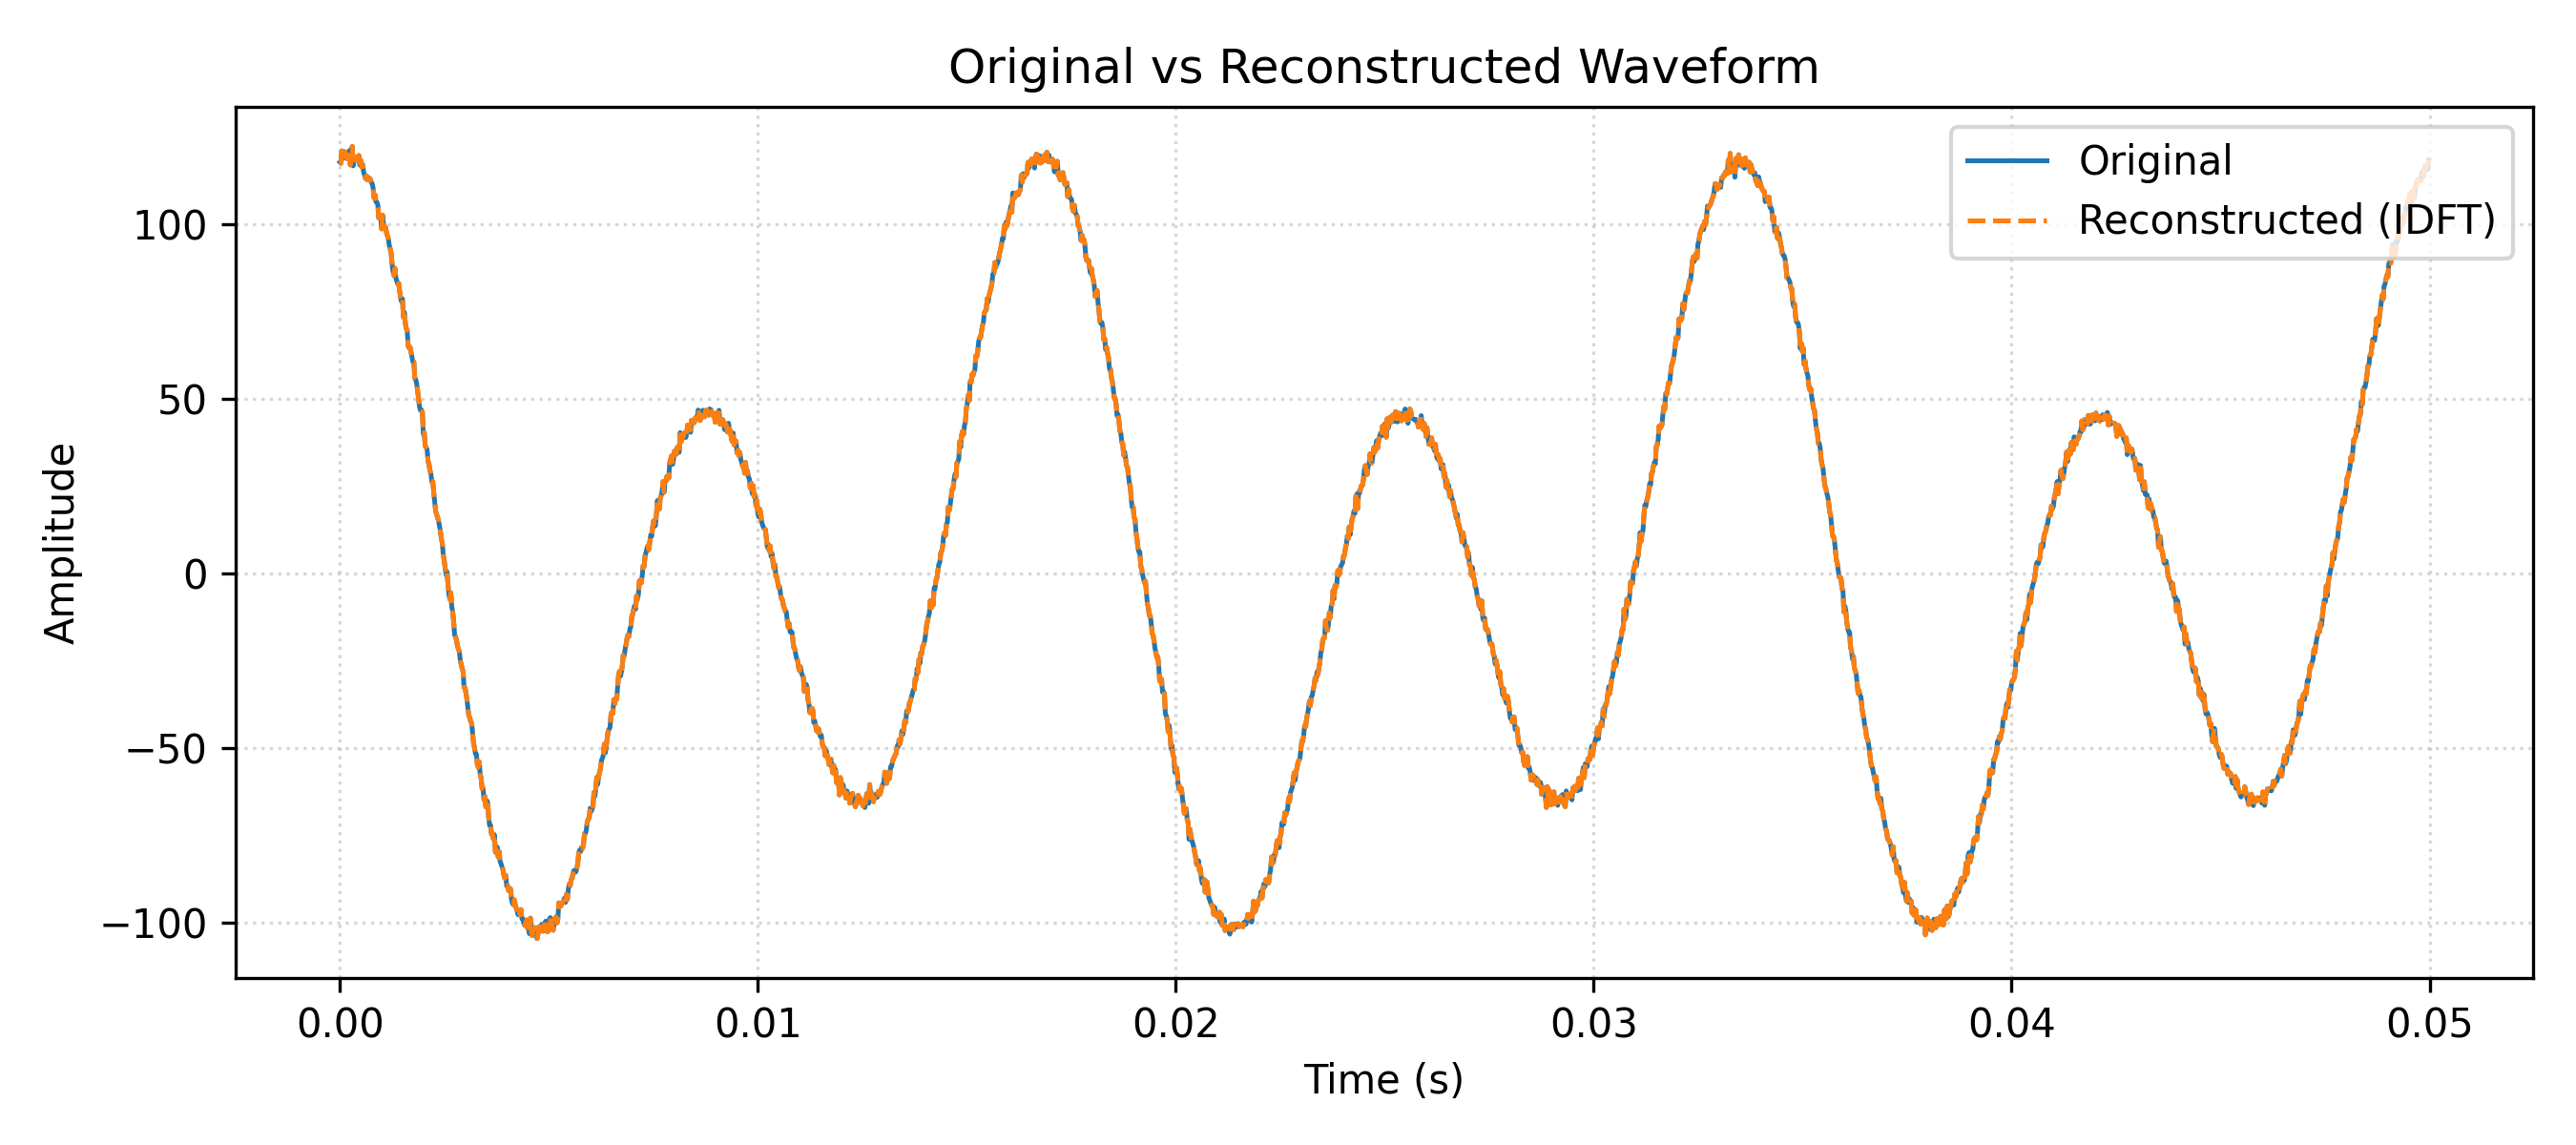
\includegraphics[width=\textwidth]{validation.png}
    \caption{A direct overlay of the original waveform and the waveform reconstructed from the Fourier coefficients.}
    \label{fig:validation}
\end{figure}

To check the accuracy numerically, I calculated the Root Mean Square Error (RMSE) between the two signals. The RMSE acts as a standard deviation of the unexplained variance, calculated across all $N=2205$ samples using the formula\footnote{This formula represents the standard deviation of the residuals, a concept directly related to the statistical variance topics in \cite{haese_math_hl}.}:
\begin{equation}
    \text{RMSE} = \sqrt{ \frac{1}{N} \sum_{n=1}^{N} (x_n - \hat{x}_n)^2 }
\end{equation}
where $x_n$ is the original sample value and $\hat{x}_n$ is the reconstructed sample value. The script output yielded:
\[ \text{RMSE} = 3.50 \times 10^{-11} \]
This validates that the DFT is an exact transformation rather than an approximation. In exact arithmetic, the RMSE would be identically zero, since the DFT and its inverse form a lossless basis transformation. The minuscule error observed is due only to computational floating-point precision.

To be sure, I plotted the leftover error (the residual) by itself. It is critical to note the scale of the y-axis on this graph: the amplitude error is on the order of $1 \times 10^{-10}$. At this microscopic scale, the error just looks like random static noise with no underlying wave pattern. As seen in Figure \ref{fig:residual_error}, the error just looks like random noise with no pattern. The spectrum of this error signal (Figure \ref{fig:residual_spectrum}) also showed no peaks, confirming that my Fourier model captured all the important deterministic parts of the signal.

\begin{figure}[H]
    \centering
    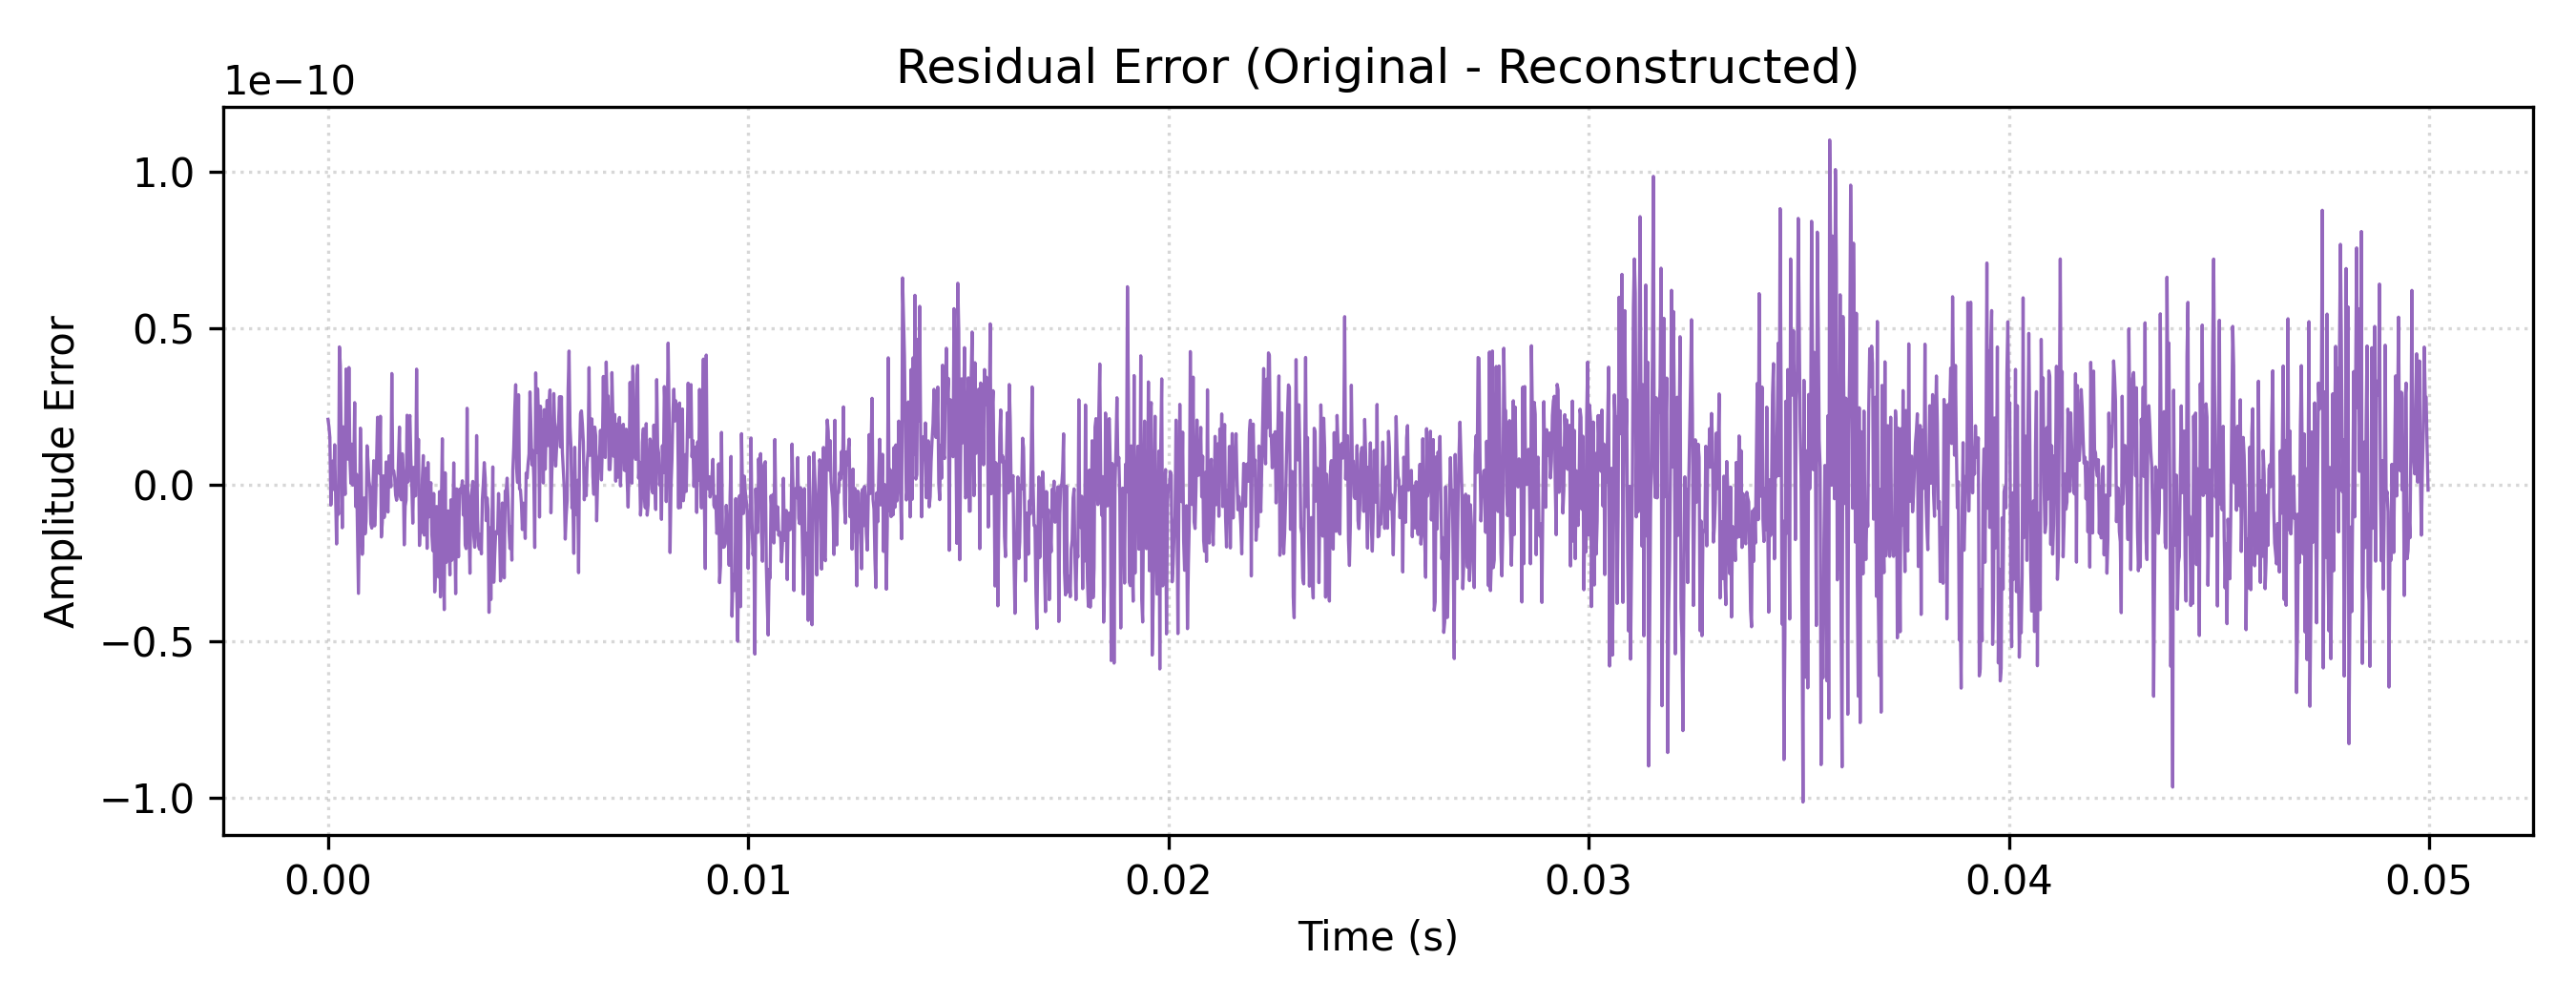
\includegraphics[width=\textwidth]{residual_error.png}
    \caption{The residual error between the original and reconstructed waveforms.}
    \label{fig:residual_error}
\end{figure}

\begin{figure}[H]
    \centering
    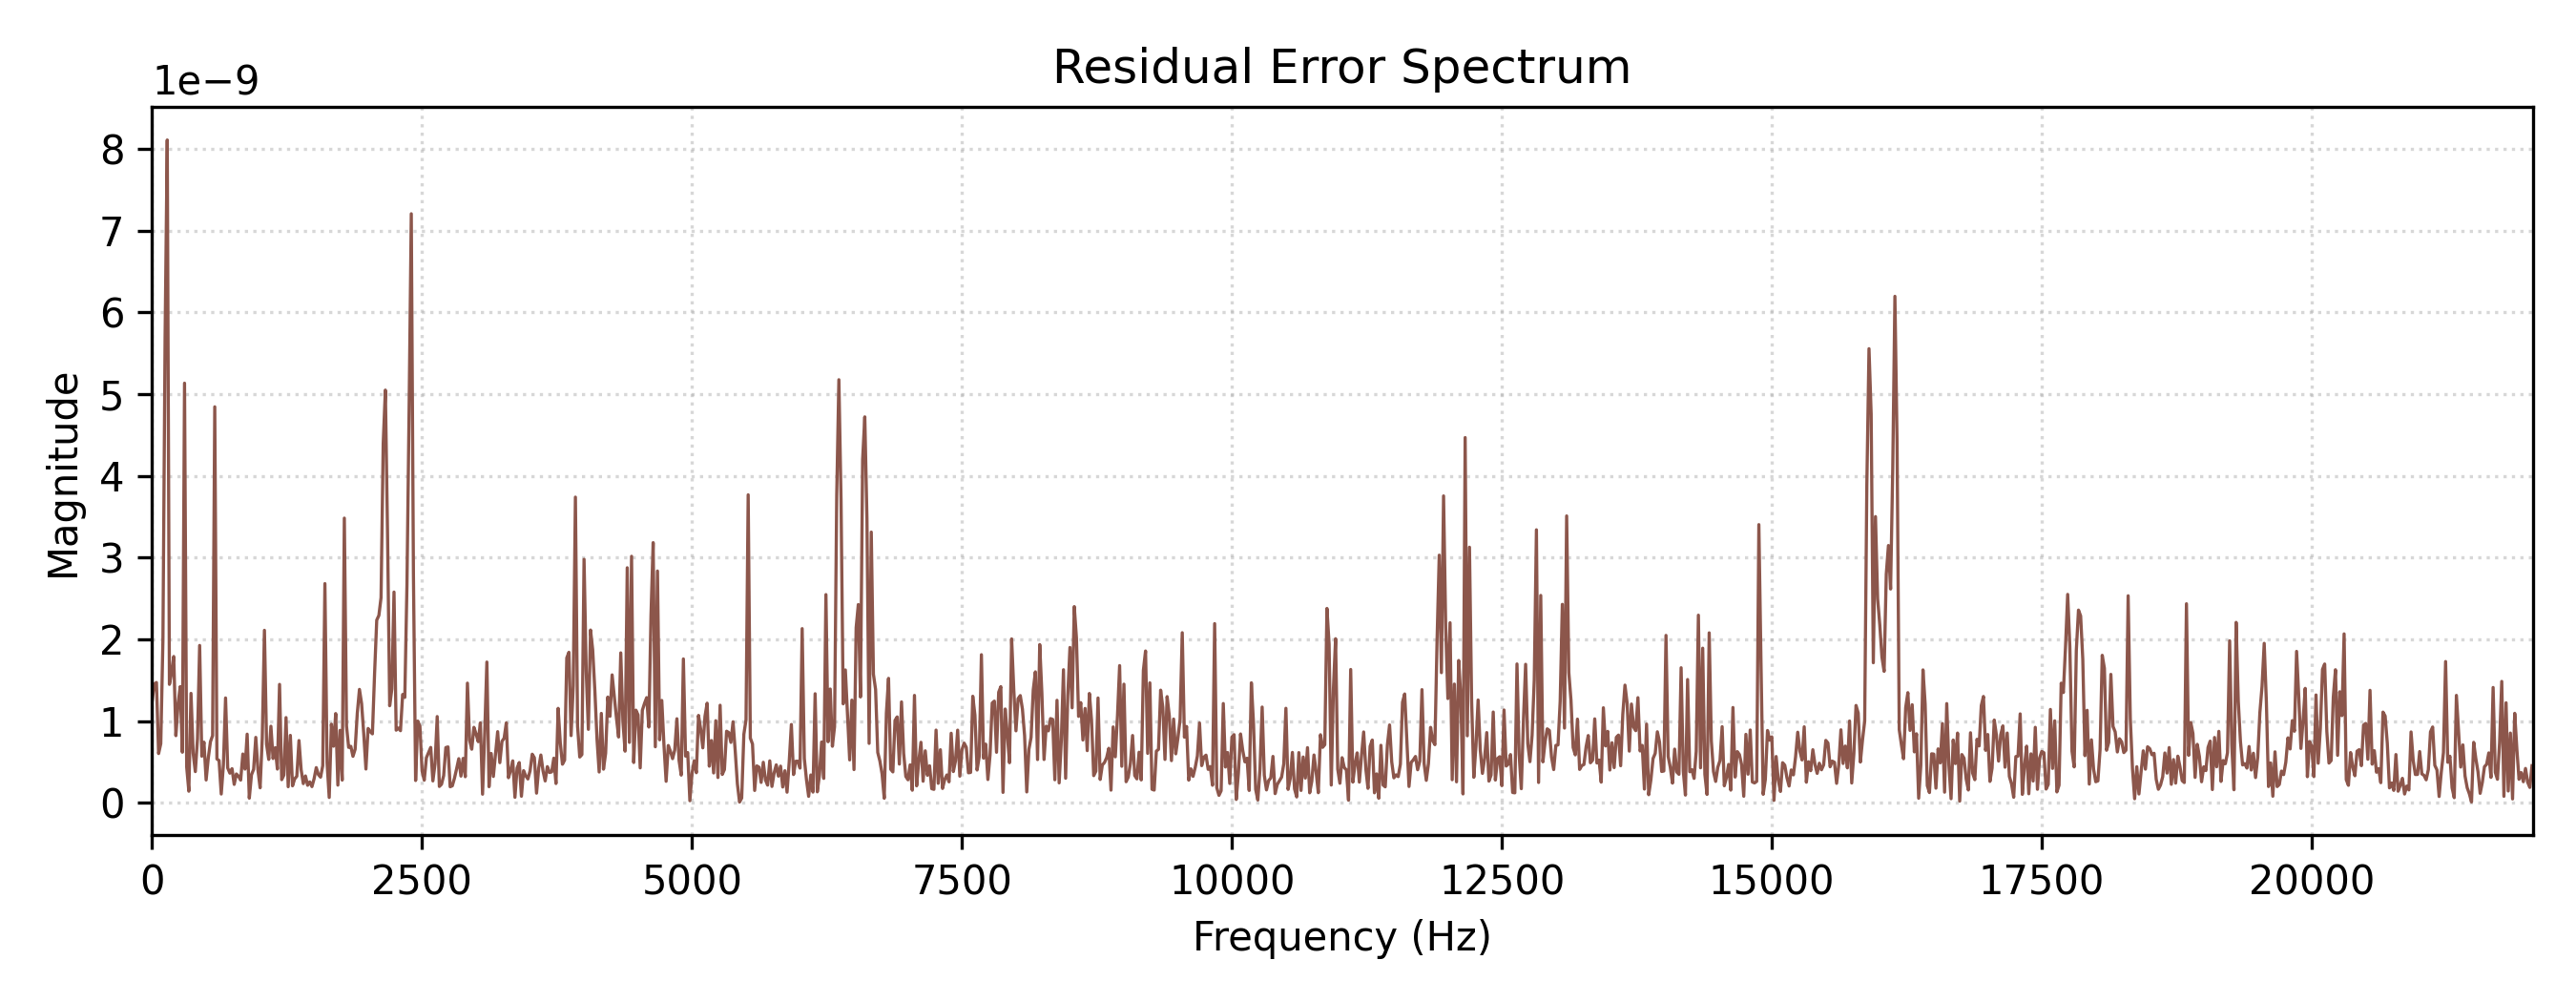
\includegraphics[width=\textwidth]{residual_spectrum.png}
    \caption{The frequency spectrum of the residual error signal.}
    \label{fig:residual_spectrum}
\end{figure}

\subsection{Interpretation of the Harmonic Structure}
The results answer my research question directly. Instead of a subjective description like warm or bright, the spectrum shows timbre as a measurable recipe of frequencies.

For this note, that recipe is defined by the specific ratio of its harmonics, especially the fact that the 120 Hz overtone dominates the 60 Hz fundamental. This is what makes it sound like a guitar and not a flute playing the same note. A flute's sound would have a much stronger fundamental and weaker harmonics. So, the Fourier analysis successfully turned the subjective quality of timbre into a clear set of numbers.

This surprising dominance of the first overtone is not a mathematical anomaly but a direct consequence of the physics of a plucked string. The relative amplitudes of harmonics are determined by the position at which the string is excited. Plucking a string precisely at its midpoint, for instance, places an antinode for the fundamental frequency there, exciting it maximally, but it also places a node for the second harmonic (first overtone), suppressing it entirely. Conversely, plucking the string at a position such as one-quarter of its length will suppress the fourth harmonic but strongly excite others. The specific harmonic recipe found in my analysis is therefore a direct fingerprint of the physical action used to produce the note, providing a deep connection between the mathematical result and the physical reality of the instrument.

% --- EVALUATION AND CONCLUSION ---
\section{Evaluation and Conclusion}

\subsection{Conclusion}
The reconstruction worked almost perfectly, showing that the mathematics lined up directly with the sound. The model was validated by an RMSE that was effectively zero, confirming that the complex waveform behaved as a superposition of simple sinusoids.

The analysis also gave a clear, mathematical answer to the question of timbre. The frequency spectrum acts as a quantitative fingerprint. For this guitar note, that fingerprint's most distinct feature was the strength of the first overtone relative to the fundamental. This shows that timbre isn't just a subjective feeling; it’s a direct result of a measurable harmonic structure.

\subsection{Strengths and Limitations}
\textbf{Strengths}
\begin{itemize}
    \item One strength was starting from first principles with the Wave Equation. It gave the whole investigation a solid theoretical backbone instead of just assuming Fourier analysis would work.
    \item Implementing the DFT algorithm manually deepened my conceptual understanding, as I could trace each computational step back to the theoretical model.
    \item Finally, analyzing the residual error instead of just relying on the RMSE gave me a deeper confidence in the model's accuracy. It showed that what was left over was just noise, not a hidden pattern the model missed.
\end{itemize}

\noindent \textbf{Limitations}
\begin{itemize}
    \item The main limitation is that the model assumes the note is perfectly periodic. A real note changes over time, and my analysis only captures a static snapshot of its timbre.
    \item The Fourier series also has trouble with sharp breaks in a signal. My wave was smooth, but if I were to analyze a more percussive sound, I would expect to see errors from the Gibbs phenomenon. This phenomenon is not merely an error but a fundamental property of uniform convergence. Near a discontinuity, any finite Fourier series will exhibit an overshoot that does not diminish in amplitude as more terms are added. This overshoot converges to a value of approximately 9 percent of the total jump height, a value related to the integral of the sinc function, $\int (\sin x)/x \,dx$ \cite{stein2003fourier}.
    \item A more comprehensive analysis would segment the waveform into attack, sustain, and decay phases, allowing comparison of how harmonic structures evolve dynamically.
\end{itemize}

\subsection{Extensions for Further Exploration}
The limitations of the static model made me curious about how to capture the full story of a sound. To see how the timbre changes over time, the next logical step would be to use the Short-Time Fourier Transform (STFT). This would let me create a spectrogram and actually watch the harmonic recipe evolve from the moment the string is plucked.

I’m also curious about applying this to sounds that aren’t notes at all, like a cymbal crash. Since these aren't periodic, the Fourier Series doesn't apply. This leads to the Fourier Transform, which works on any signal. Exploring these tools would be the next step in using math to understand the structure of any sound, not just a simple, static note.
\newpage
% --- REFERENCES ---
\begin{thebibliography}{9}

\bibitem{haese_aa_hl} Haese, M., Humphries, M., et al. (2019). \textit{Mathematics: Analysis and Approaches HL}. Haese Mathematics.
\bibitem{halliday_resnick} Halliday, D., Resnick, R., \& Walker, J. (2013). \textit{Fundamentals of Physics} (10th ed.). Wiley.
\bibitem{iowa} University of Iowa Electronic Music Studios. (n.d.). \textit{Musical Instrument Samples}. Retrieved from \url{https://theremin.music.uiowa.edu/MISguitar.html}
\bibitem{stein2003fourier} Stein, E. M., \& Shakarchi, R. (2003). \textit{Fourier Analysis: An Introduction}. Princeton University Press.
\bibitem{haese_math_hl} Urban, P., Martin, D., et al. (2012). \textit{Mathematics for the international student: Mathematics HL (Core)}. Haese \& Harris Publications.
\bibitem{3b1b} 3Blue1Brown. (2019, June 2). \textit{But what is the Fourier Transform? A visual introduction}. [Video]. YouTube. \url{https://www.youtube.com/watch?v=spUNpyF58BY}
\bibitem{gemini2026} Google Gemini(2026). \textit{Gemini 3.1 Pro}. Large language model used for coding assistance. https://gemini.google.com/

\end{thebibliography}

% --- APPENDICES ---
\newpage
\section*{Appendices}
\appendix
\section{Python Implementation Code}
This code was written in Python to process the guitar waveform used in my investigation. It loads the audio file, isolates a short stable segment of a single note, and then applies a manual Discrete Fourier Transform (DFT) to calculate the harmonic coefficients. The script also plots the spectrum, finds the dominant peaks, reconstructs the waveform using the inverse transform, and measures the error between the original and reconstructed signals. The manual DFT is included here because it directly shows the summation formula used in my mathematical model, even though in practice a fast algorithm (FFT) would normally be used.

\begin{lstlisting}[language=Python, caption=Full Python code for DFT analysis and reconstruction.]
# appendix code - manual DFT and reconstruction

Note: The structural framework and debugging of this Python script were assisted by AI (Google Gemini 3.1 Pro.)

import numpy as np
from scipy.io import wavfile
import matplotlib.pyplot as plt
from scipy.signal import find_peaks

# load wav file
filename=Guitar_sample.wav
samplerate,data=wavfile.read(filename)

# convert stereo to mono if needed
if data.ndim==2:
    data=data.mean(axis=1)

# plot full waveform
duration=len(data)/samplerate
time_axis_full=np.linspace(0,duration,len(data),endpoint=False)

plt.figure(figsize=(12,3))
plt.plot(time_axis_full,data)
plt.title(full waveform)
plt.xlabel(time (s))
plt.ylabel(amplitude)
plt.show()

# cut one note out
note_start=int(2.0*samplerate); note_end=int(4.0*samplerate)
single_note=data[note_start:note_end]
time_note=np.linspace(2.0,4.0,len(single_note))

plt.figure()
plt.plot(time_note,single_note)
plt.title(note event)
plt.show()

# short stable slice
seg_start=int(2.1*samplerate)
seg_end=int((2.1+0.05)*samplerate)
segment=data[seg_start:seg_end]
time_seg=np.linspace(0,0.05,len(segment))

plt.plot(time_seg,segment)
plt.title(segment for analysis)
plt.show()

# manual DFT (slow but shows formula)
N=len(segment)
manual_dft=np.zeros(N,dtype=complex)
for k in range(N):
    s=0
    for n in range(N):
        angle=-2*np.pi*k*n/N
        s+=segment[n]*np.exp(1j*angle)
    manual_dft[k]=s

freqs=np.fft.fftfreq(N,d=1/samplerate)
mags=np.abs(manual_dft)

# find peaks in spectrum
peaks,_=find_peaks(mags,prominence=np.max(mags)*0.05)
pos_peaks=peaks[freqs[peaks]>=0]

print(peaks detected:)
for p in pos_peaks:
    print(freqs[p],mags[p])

plt.plot(freqs,mags)
plt.scatter(freqs[pos_peaks],mags[pos_peaks],color=red)
plt.xlim(0,3000)
plt.title(spectrum)
plt.show()

# inverse transform + error check
reconstructed=np.fft.ifft(manual_dft).real
rmse=np.sqrt(np.mean((segment-reconstructed)**2))
print(rmse:,rmse)

residual=segment-reconstructed
plt.plot(time_seg,residual)
plt.title(residual)
plt.show()

# residual spectrum
res_fft=np.fft.fft(residual)
res_freq=np.fft.fftfreq(N,d=1/samplerate)
plt.plot(res_freq,np.abs(res_fft))
plt.xlim(0,samplerate/2)
plt.title(residual spectrum)
plt.show()

# final overlay
plt.plot(time_seg,segment,label=orig)
plt.plot(time_seg,reconstructed,--,label=recon)
plt.legend(); plt.title(original vs reconstructed)
plt.show()
import numpy as np
import matplotlib.pyplot as plt

def plot_aliasing():
    plt.figure(figsize=(10, 4))
    
    # The true, high-frequency continuous signal (e.g., 9 Hz)
    t_continuous = np.linspace(0, 1, 500)
    true_signal = np.sin(2 * np.pi * 9 * t_continuous)
    
    # The low sampling rate (e.g., 10 Hz)
    fs = 10
    t_discrete = np.linspace(0, 1, fs + 1)
    discrete_samples = np.sin(2 * np.pi * 9 * t_discrete)
    
    # The resulting aliased low-frequency signal (appears as -1 Hz)
    aliased_signal = np.sin(2 * np.pi * -1 * t_continuous)
    
    # Plotting
    plt.plot(t_continuous, true_signal, 'b-', alpha=0.4, label='True High-Frequency Signal (9 Hz)')
    plt.plot(t_continuous, aliased_signal, 'r--', linewidth=2, label='Perceived Aliased Signal (-1 Hz)')
    plt.plot(t_discrete, discrete_samples, 'ko', markersize=8, label=f'Discrete Samples (sampled at {fs} Hz)')
    
    # Formatting
    plt.title('Visualizing the Nyquist Limit: Signal Aliasing')
    plt.xlabel('Time [s]')
    plt.ylabel('Amplitude')
    
    # FIX: Expand the y-axis so the legend doesn't cover the wave peak
    plt.ylim(-1.2, 2.0)
    
    plt.legend(loc='upper right', framealpha=0.9)
    plt.grid(True, linestyle=':', alpha=0.7)
    plt.tight_layout()
    plt.savefig('aliasing_diagram.png', dpi=300)
    plt.show()

plot_aliasing()

import numpy as np
import matplotlib.pyplot as plt

# ==========================================
# DIAGRAM 1: Riemann Sum Approximation
# ==========================================
def plot_riemann_sum():
    plt.figure(figsize=(8, 5))
    
    # Create a generic continuous curve
    t_continuous = np.linspace(0, 1, 200)
    f_continuous = np.sin(2 * np.pi * t_continuous) * np.exp(-t_continuous) + 1.5
    
    # Create discrete sample points (N=10 for visual clarity)
    N = 10
    t_discrete = np.linspace(0, 1, N, endpoint=False)
    f_discrete = np.sin(2 * np.pi * t_discrete) * np.exp(-t_discrete) + 1.5
    dt = 1/N
    
    # Plot the continuous curve
    plt.plot(t_continuous, f_continuous, 'b-', linewidth=2, label='Continuous function $f(t)e^{-ik\omega_0t}$')
    
    # Plot the discrete rectangles
    plt.bar(t_discrete, f_discrete, width=dt, alpha=0.4, color='orange', align='edge', edgecolor='black', label='Discrete samples (Riemann slices)')
    
    # Formatting
    plt.title('Riemann Sum Approximation from Continuous to Discrete')
    plt.xlabel('Time (t)')
    plt.ylabel('Amplitude')
    plt.legend()
    plt.grid(True, linestyle='--', alpha=0.6)
    plt.savefig('riemann_sum.png', dpi=300, bbox_inches='tight')
    plt.show()

# ==========================================
# DIAGRAM 2: DFT Complex Unit Circle
# ==========================================
def plot_unit_circle():
    plt.figure(figsize=(6, 6))
    
    # Draw the unit circle
    angles = np.linspace(0, 2 * np.pi, 100)
    plt.plot(np.cos(angles), np.sin(angles), 'k--', alpha=0.5)
    
    # The 4 points for N=4
    n_values = [0, 1, 2, 3]
    labels = [r'$e^0 = 1$', r'$e^{-i\pi/2} = -i$', r'$e^{-i\pi} = -1$', r'$e^{-i3\pi/2} = i$']
    colors = ['red', 'blue', 'green', 'purple']
    
    # Plot points and arrows
    for n, label, color in zip(n_values, labels, colors):
        angle = -np.pi * n / 2
        x, y = np.cos(angle), np.sin(angle)
        
        # Draw vector arrow
        plt.quiver(0, 0, x, y, angles='xy', scale_units='xy', scale=1, color=color, width=0.008)
        
        # Plot the dot
        plt.plot(x, y, 'ko')
        
        # Add label slightly offset
        plt.text(x * 1.2, y * 1.2, label, fontsize=12, ha='center', va='center', 
                 bbox=dict(facecolor='white', edgecolor='none', alpha=0.7))

    # Formatting
    plt.axhline(0, color='black', linewidth=1)
    plt.axvline(0, color='black', linewidth=1)
    plt.xlim(-1.5, 1.5)
    plt.ylim(-1.5, 1.5)
    plt.title('DFT Complex Exponentials ($N=4$)')
    plt.xlabel('Real Axis (Re)')
    plt.ylabel('Imaginary Axis (Im)')
    plt.grid(True, linestyle=':', alpha=0.6)
    plt.gca().set_aspect('equal', adjustable='box')
    plt.savefig('unit_circle_roots.png', dpi=300, bbox_inches='tight')
    plt.show()

# Run both functions
plot_riemann_sum()
plot_unit_circle()
\end{lstlisting}




\end{document}